\documentclass[useAMS,usenatbib]{mn2e}

\usepackage{natbib}
\usepackage{graphicx}
\usepackage{color}
\usepackage{amssymb}
\usepackage{amsmath}
\usepackage{xspace}
\usepackage{xargs}

\usepackage[usenames,dvipsnames]{xcolor}
\definecolor{FireBrick}{RGB}{178, 34, 34}

\usepackage[usenames,dvipsnames]{xcolor}
\newcommand{\spb}[1]{{\bf \textcolor{blue}{SPB: #1}}}
\newcommand{\rk}[1]{{\bf \textcolor{ForestGreen}{RK: #1}}}
\newcommand{\rh}[1]{{\bf \textcolor{RoyalPurple}{RH: #1}}}

%%%%%%%%%%%%%%%%%
\newcommand{\galfit}{{\scshape galfit}\xspace}
\newcommand{\galfitthree}{{\scshape galfit3}\xspace}
\newcommandx{\N}[2][1= ,2= ]{$\mathcal{N}^{#1}_{#2}$\xspace}
\newcommandx{\R}[2][1= ,2= ]{$\mathcal{R}^{#1}_{#2}$\xspace}
\newcommand{\re}{R_{\rm e}}

\begin{document}
\title[Galaxy Zoo: debiasing and spiral arm number]{Galaxy Zoo: improved debiasing for multiple-answer questions and the demographics of spiral arm number}
\author[Hart et al.]{Ross~E.~Hart$^1$\thanks{E-mail: ross.hart@nottingham.ac.uk}, Steven~P.~Bamford$^1$ and the Galaxy Zoo team
\smallskip\\
$^{1}$School of Physics \& Astronomy, The University of Nottingham, University Park, Nottingham, NG7 2RD, UK\
}
\maketitle
\begin{abstract}
Here we study the behaviour...
``climbing the question tree''
\end{abstract}

\begin{keywords}
galaxies: general -- galaxies: structure -- galaxies: fundamental parameters -- galaxies: formation
\end{keywords}

%------------------------------------------------------------------------------------
%%%%%%%%%%%%%%%%%%%%%%%%%%%%%%%%%%%%%%%%%%%%%%%%%%%%%%%%%%%%%%%%%%%%%%%%%%%%%%%%%%%%%
%------------------------------------------------------------------------------------
\section{Introduction}
\label{sec:intro}
Spiral galaxies are the most common type of galaxy in the local Universe \citep{Lintott_11,Willett_13}, yet formulating a single theory to account for all spiral structure still remains elusive. As most local Universe star-formation is associated with spiral galaxies, and spiral arms themselves are sites of enhanced stellar density, understanding spiral structure is key to understanding the  star-formation of the local Universe. The main theories for the occurrence of spiral arm features in local galaxies initially focused on the idea of being caused by density waves in their disks \citep{Lindblad_63,Lin_64}, but have since been preceded by theories that consider the effects of gravity and disk dynamics \citep{Toomre_81,Sellwood_84}, with most if the work to advance the field of spiral structure theory being driven by simulations. Using observational studies to test these theories remains a challenge, as visual classifications of both the presence of spiral structure and its detailed features are required, which are difficult to obtain when considering the large samples provided by galaxy survey data.

An approach that has been used to visually classify galaxies in large survey samples has been to utilise citizen science, by allowing volunteers to morphologically classify galaxies rather than relying on classifications from a small number of experts. Galaxy Zoo 1 (GZ1, \citealt{Lintott_08,Lintott_11}) was the first project to collect visual morphologies in this way, by classifying galaxies from the Sloan Digital Sky Survey (SDSS) as either `smooth' or `spiral'. Using this method, each galaxy is classified by several individuals, and a likelihood or `vote fraction' of each galaxy having a particular feature is assigned as the fraction of classifiers who claimed they saw that feature. GZ1 classifications collected in this way have been used to compare galaxy morphology with respect to colour \citep{Masters_10a,Masters_10b,Bamford_09}, environment \citep{Skibba_09,Bamford_09}, and star-formation properties \citep{Tojeiro_13,Schawinski_14,Smethurst_15}. 

Following from the success of GZ1, more detailed visual classifications were sought, looking for a much more comprehensive set of classifications of features that galaxies exhibit in the local Universe, including the presence of bars, and spiral arm winding and multiplicity properties. Thus, Galaxy Zoo 2 was created (GZ2,\citealt{Willett_13}, hereafter W13), in which volunteers were asked more questions about a subsample of SDSS galaxies than in GZ1. The main difference between GZ2 and GZ1 was that visual classifications were collected using a `question tree' in GZ2, to gain a more exhaustive set of morphological information for each galaxy. GZ2 has already been used as a measure for detailed galaxy morphology, for example being used to compare the properties of spiral galaxies with or without bars \citep{Masters_11,Masters_12,Cheung_13}, look for interacting galaxies \citep{Casteels_13}, as well as looking for relationships between spiral arm structure and star-formation \citep{Willett_15}. This `question tree' method has since been used in a similar way to measure the presence of detailed morphological features in higher redshift galaxy surveys (see \citealt{Melvin_14} and \citealt{Simmons_14} for examples), and other \textsc{Zooniverse} citizen science projects. 

An issue that arises in both visual and automated methods of morphological classification is that detailed features are more difficult to observe in lower signal-to-noise images observed from a greater distance. In Galaxy Zoo, this has been termed as classification bias. It is imperative that classification bias is removed from morphological data, as it leads to sample contamination. This means that any observational differences between samples can be significantly reduced.

Classification bias manifested itself in GZ1 with galaxies at higher redshift having lower `spiral' vote fractions, which were corrected using a numerical method \citep{Bamford_09}. The application of a question tree in GZ2 to look for more detailed features means that correcting for biases is more complicated than in GZ1. In particular, there are questions with several possible answers, and debiasing one answer with respect to each of the others is therefore a less trivial process in GZ2.

The paper is organised as follows. In section 2, the sample selection and galaxy data are described. In section 3, we describe a new debiasing method that has been created to account for the classification bias in the GZ2 questions with multiple possible answers. In section 4, samples of GZ2 spiral galaxies are defined and sorted by arm multiplicity, a case where the new debiasing method is required as there are multiple responses to that question. The overall demographics of these galaxies are then compared with respect to arm multiplicity, in order for us to look for clues as to what processes influence their formation and evolution. The results are summarised in section 5.
%------------------------------------------------------------------------------------
%%%%%%%%%%%%%%%%%%%%%%%%%%%%%%%%%%%%%%%%%%%%%%%%%%%%%%%%%%%%%%%%%%%%%%%%%%%%%%%%%%%%%
%------------------------------------------------------------------------------------
\section{Data}
\label{sec:data}
%------------------------------------------------------------------------------------
\subsection{Galaxy properties and sample selection}
\label{sec:sample}

We make use of morphological information from the public data release of Galaxy Zoo 2 (GZ2; W13). The galaxies classified by GZ2 were taken from the Sloan Digital Sky Survey (SDSS) Data Release 7 (DR7; \citealt{Abazijian_09}). The GZ2 sample contains essentially all well-resolved galaxies in DR7 down to a limiting absolute magnitude of $m_r \leq 17$, supplemented by additional sets of galaxies in Stripe 82 for which deeper, co-added imaging exists (see W13 for details).  In this paper we only consider galaxies with $m_r \leq 17$ that were classified in normal-depth SDSS imaging and which have DR7 spectroscopic redshifts. We refer to this as our \textit{full sample}, containing $228,201$ galaxies, to which the debiasing procedure described in \S~\ref{sec:new_method} is applied. We require redshifts in order to correct the sample for a distance-dependent bias, as described in \S~\ref{sec:biases}.

Petrosian aperture photometry in $ugriz$ filters is obtained from the SDSS DR7 catalogue. Rest-frame absolute magnitudes are those computed by \citet{Bamford_09}, using \textsc{kcorrect} \citep{Blanton_07}. Galaxy stellar masses are determined from the $r$-band luminosity and $u-r$ colour using the calibration adopted by \citet{Baldry_06}.
All relevant quantities assume a flat cosmology with $\Omega_\mathrm{m} = 0.3$ and $H_0 = 70\;\mathrm{km\,s^{-1}\,Mpc^{-1}}$.

In order to study galaxy properties in a representative manner in \S~\ref{sec:results}, we define a \textit{luminosity-limited sample} with $0.03<z<0.085$ and $M_r \le -21$, containing $62,220$ galaxies. The luminosity versus redshift distribution of our \textit{full sample}, and the limits of our \textit{luminosity-limited sample}, are shown in Fig.~\ref{fig:vl_sample}.  These limits approximately maximize the sample size, given the $m_r \le 17$ limit on the \textit{full sample}. The lower redshift limit avoids a small number of galaxies with very large angular sizes, and hence accompanying morphological, photometric and spectroscopic complications. The upper redshift limits also corresponds to that for which we have reliable galaxy environmental density data from \cite{Baldry_06}, which we will make use of in this paper.  

\begin{figure}
		\centering
		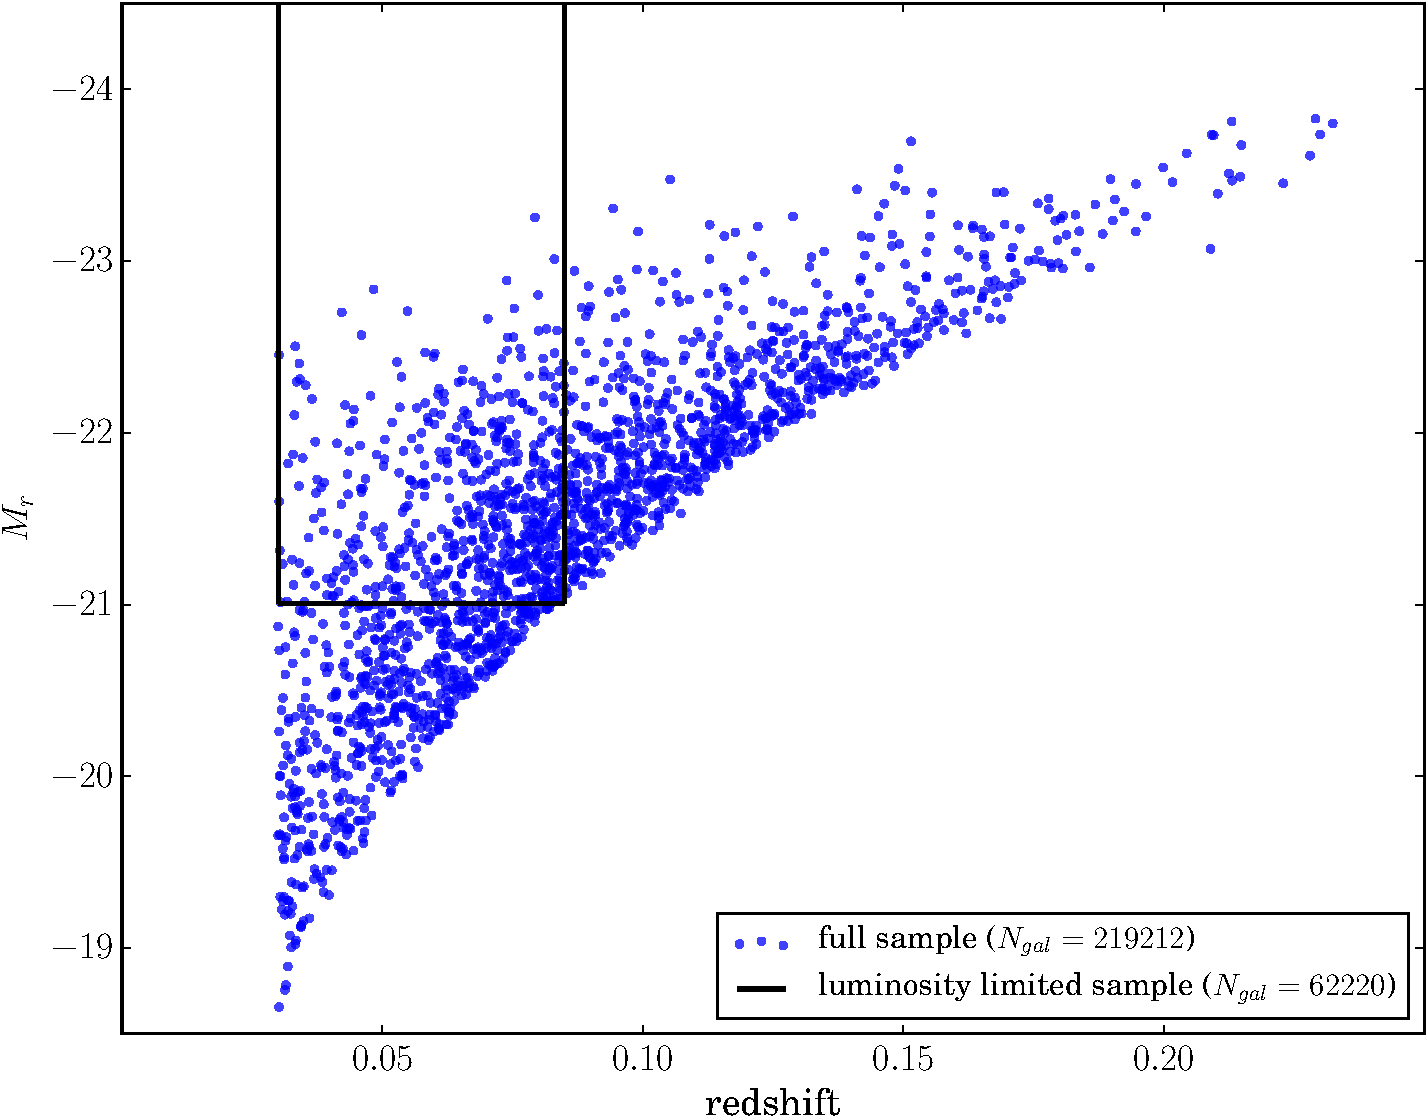
\includegraphics[width=0.45\textwidth]{Images/Data/volume_limited_sample-crop.pdf}
    \caption{The $r$-band luminosity versus redshift distribution of our \textit{full sample} (blue points), with the region enclosing our $0.03<z<0.085$, $M_r  \leq -21$ \textit{luminosity-limited sample} indicated by black lines. Only a random selection of 2000 points are plotted for clarity.
		\label{fig:vl_sample}}
\end{figure}

In terms of stellar mass, the \textit{luminosity-limited sample} is incomplete for the reddest galaxies at $\log (M/M_{\odot}) < 10.6$. Where necessary we therefore consider a \textit{stellar mass-limited sample} of 41,801 galaxies, created by applying a limit of $\log (M/M_{\odot}) \geq 10.6$ to the \textit{luminosity-limited sample}.
%------------------------------------------------------------------------------------
\subsection{Stellar population models}
\label{sec:SEDs}

In \S~\ref{sec:colours}, star-formation histories (SFHs) are compared to stellar population models. Spectral energy distributions (SEDs) are derived from \citealt{BC_03}, for a range of ages and SFHs using the initial mass function from \citealt{Chabrier_03}. For the models described in this paper, a single metallicity value of $Z=Z_{\odot}$ is used. Two dust extinction magnitudes of $A_v$=0 and $A_v$=0.4 are considered, derived in \citealt{Calzetti_00}. Equivalent colours for each of the star-formation and dust extinction models are calculated for each of the SDSS $ugriz$ filters, with the wavelength dependent filter opacities measured in \citealt{Doi_10}. Full details of how the models are derived can be found in \citealt{Duncan_14}.
%------------------------------------------------------------------------------------
\subsection{Quantifying morphology with Galaxy Zoo}
\label{sec:gz_morphologies}

In GZ2, morphological information for each galaxy was obtained by asking participants to answer a series of questions. The structure of this question tree is shown in Fig.~\ref{fig:question_tree}. Typically, each image was viewed by $\ga 40$ people (W13), but each of the questions is not answered about each galaxy. The questions further down the question tree require that another question has been answered with a particular response. For each question, the responses are each represented by the `vote fraction`, $p$ assigned to each possible answer. For any given question, the sum of the $p$-values for all possible answers adds up to 1. Considering the `edge-on' question (T01 in Fig.~\ref{fig:question_tree}), a classifier would only answer that question if they had already said that they had saw features. If a galaxy was classified by 40 people, and 30 of those said they saw features, whilst the other 10 claimed it was smooth, then the corresponding $p$-values are $p_{\mathrm{features}}=0.75$ and $p_\mathrm{{smooth}}=0.25$. Only the 30 classifiers who saw `features' then answered the `spiral' question. If 15 of those said the galaxy was edge-on, and 15 said it was not, the corresponding $p$-values would be $p_{edge-on}=0.5$ and $p_{not \, edge-on}=0.5$. 

In order to reduce the influence of unreliable classifiers, W13 down-weighted individual volunteers who had poor agreement.  Throughout this paper we refer to these weighted vote fractions as the `raw' quantities. Before using these GZ2 vote fractions to study the galaxy population, we must first consider the issue of classification bias, as we shall in \S~\ref{sec:biases}.

\begin{figure}
		\centering
		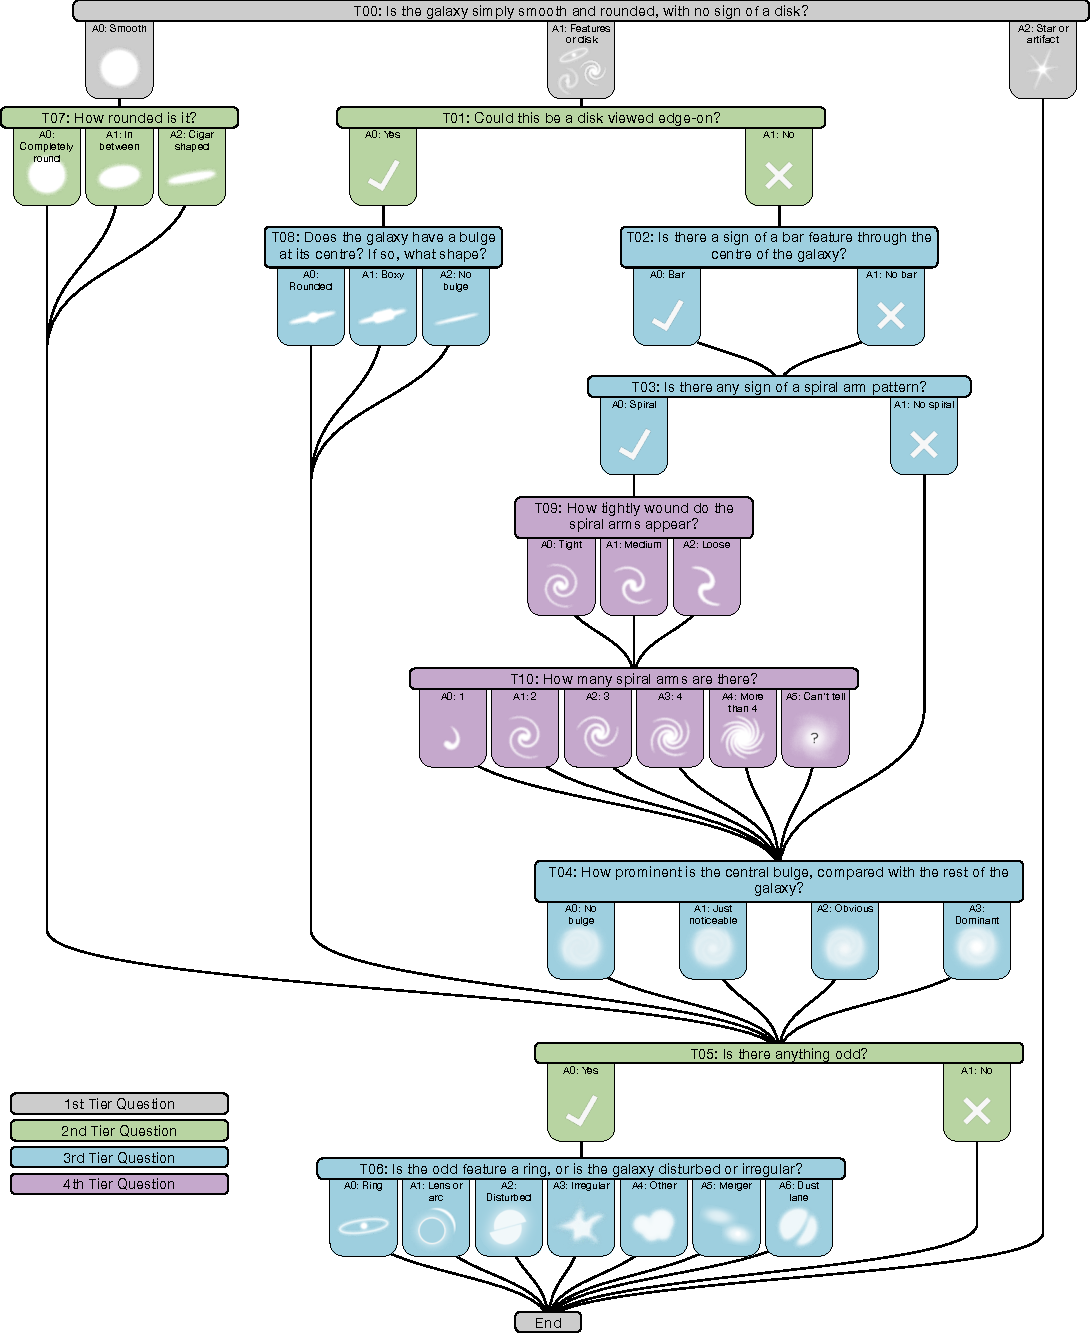
\includegraphics[width=0.5\textwidth]{Images/Data/gz2_tree_crop.pdf}
    \caption{Diagram of the question tree that is used to classify galaxies in GZ2. The tasks are colour-coded by their depth in the question tree. As an example, the arm number question is a fourth tier question- to answer that particular question about a given galaxy, they need to have given a particular response to three previous questions (that the galaxy had features, was not edge-on and had spiral arms).}
    \label{fig:question_tree}
\end{figure}

Traditional morphologies assign each galaxy to a specific class, usually determined by one, or occasionally a few, experts. In contrast, Galaxy Zoo provides a large number of independent opinions on specific morphological features for each galaxy.  This allows us to consider both the inherent `fuzziness' and observational uncertainties of galaxy morphology, and hence control the compromise between sample contamination and completeness.

There are two principal ways in which galaxy morphologies can be quantified using Galaxy Zoo vote fractions. The first is to consider averages of the vote fractions over specific samples or bins divided by some other property.  These average vote fractions can then be used to study variations in the morphological content of the galaxy population.  Individual galaxies are not given specific classifications.  There is no population of `unclassified', and hence ignored, galaxies.  This approach has been taken by \citet{Bamford_09}, \citet{Casteels_13}, \citet{Willett_15}, and various other studies. With this method, the vote fractions of all galaxies can be considered together; even galaxies with a small (but non-zero) vote fraction for a given property count towards the statistics. Effectively, this approach considers the vote fractions as an estimate of the probability of a galaxy belonging to a particular class.

The second approach is to divide the galaxy sample in to different morphological categories, either by applying a threshold on the vote fractions, or choosing the class with the largest vote fraction. Such methods have been used by \citet{Land_08}, \citet{Skibba_09}, and many more.  One advantage of this approach is that each galaxy is assigned to a definite class, with the threshold tuned to ensure a desired level of classification certainty.  However, a set of `uncertain' or `unclassified' galaxies may remain.  In some analyses these will require special attention.

These different approaches are also relevant for how questions at different levels in the tree are combined.  For example, a participant is only asked if they can see spiral arms when they have already answered that they can see features in the galaxy and that the galaxy is not an edge-on disc.  The vote fraction for spiral arms therefore represents the conditional probability of spiral arms \emph{given that} features are discernible \emph{and} that the galaxy is not edge-on. When considering whether a galaxy displays spiral arms, one should account for the answers to these previous questions in the tree.  One can treat vote fractions as probabilities, multiplying them to obtain a `probability' that a galaxy displays any features, is not edge-on and possesses spiral arms.  Alternatively, one may select a set of galaxies that display features and are not edge-on and possess spiral arms, by applying some thresholds to the vote fractions for each question in turn. (See \citealt{Casteels_13} for a more thorough discussion of these issues.)

The primary morphological feature we will focus on in this paper is the apparent number of spiral arms displayed by a galaxy.  As we will see, some of the classes for this feature contain a relatively low fraction of the total spiral population.  In addition, the vote fractions for the preferred answer are often fairly low, with votes distributed over several answers.  In such cases, averaging the vote fractions over the full sample does not work particularly well, as noise from more common galaxy classes overwhelms the subtle signal from rarer classes.  In this paper we therefore prefer to assign galaxies to morphological samples by applying a threshold or taking the answer with the largest vote fraction.

%------------------------------------------------------------------------------------
%%%%%%%%%%%%%%%%%%%%%%%%%%%%%%%%%%%%%%%%%%%%%%%%%%%%%%%%%%%%%%%%%%%%%%%%%%%%%%%%%%%%%
%------------------------------------------------------------------------------------
\section{Correcting for redshift-dependent classification bias}
\label{sec:redshift_bias}
%------------------------------------------------------------------------------------
\subsection{Biases in the Galaxy Zoo sample}
\label{sec:biases}

Due to their distance, galaxies at high redshift appear fainter in the SDSS images than galaxies at lower redshift, and therefore have lower signal-to-noise. This means that more detailed features may be more difficult to distinguish in galaxies at higher redshift. It should also be noted that such biases are not exclusive to Galaxy Zoo. Difficulty in observing faint features in lower signal-to-noise galaxies is an inherent property of any visual or automated method of galaxy classification. The advantage of using Galaxy Zoo classifications is that it gives us a statistical method of looking at galaxy morphologies. As each of the galaxies in the full galaxy sample has been visually classified by a number of independent observers, the apparent evolution in the presence of features can be modelled, and any bias can be corrected accordingly.

Sample incompleteness and sample contamination are defects that arise in a sample where an inherent redshift bias affects the classifications.  Sample incompleteness affects the `harder to see' features- the fraction of galaxies classified as having a particular feature decreases with redshift, leaving us with poor number statistics for a sample we wish to define as having that feature.  Sample contamination is the converse effect that appears in the `easier to see' categories.  In this case, the samples defined using the Galaxy Zoo classifications also include mis-classified galaxies that should have actually been included in one of the `harder to see' categories. Any intrinsic differences between samples that one wishes to compare may be therefore be negated.

The effect of redshift bias is shown in Fig.~\ref{fig:vote_histograms}a, where the features answer to the smooth or features question is considered for a  high and low-redshift \textit{luminosity-limited sample}. The redshift range of the SDSS sample is shallow enough to justify that there should be minimal change in the overall population of galaxies \citep{Bamford_09,Willett_13}. In a \textit{luminosity-limited sample}, the level of completeness should also be the same at all redshifts, meaning that the overall populations of the high and low redshift samples should be equivalent. However, a greater fraction of the galaxies have lower values for $p_{features}$ in the higher redshift sample, as classifiers have greater difficulty picking out features in the lower signal-to-noise images. If one wished to compare a sample of galaxies with `features' against one that is `smooth' using the raw vote fractions, the number of galaxies with `features' would be incomplete and the `smooth' sample would be contaminated.

\begin{figure}
		\centering

        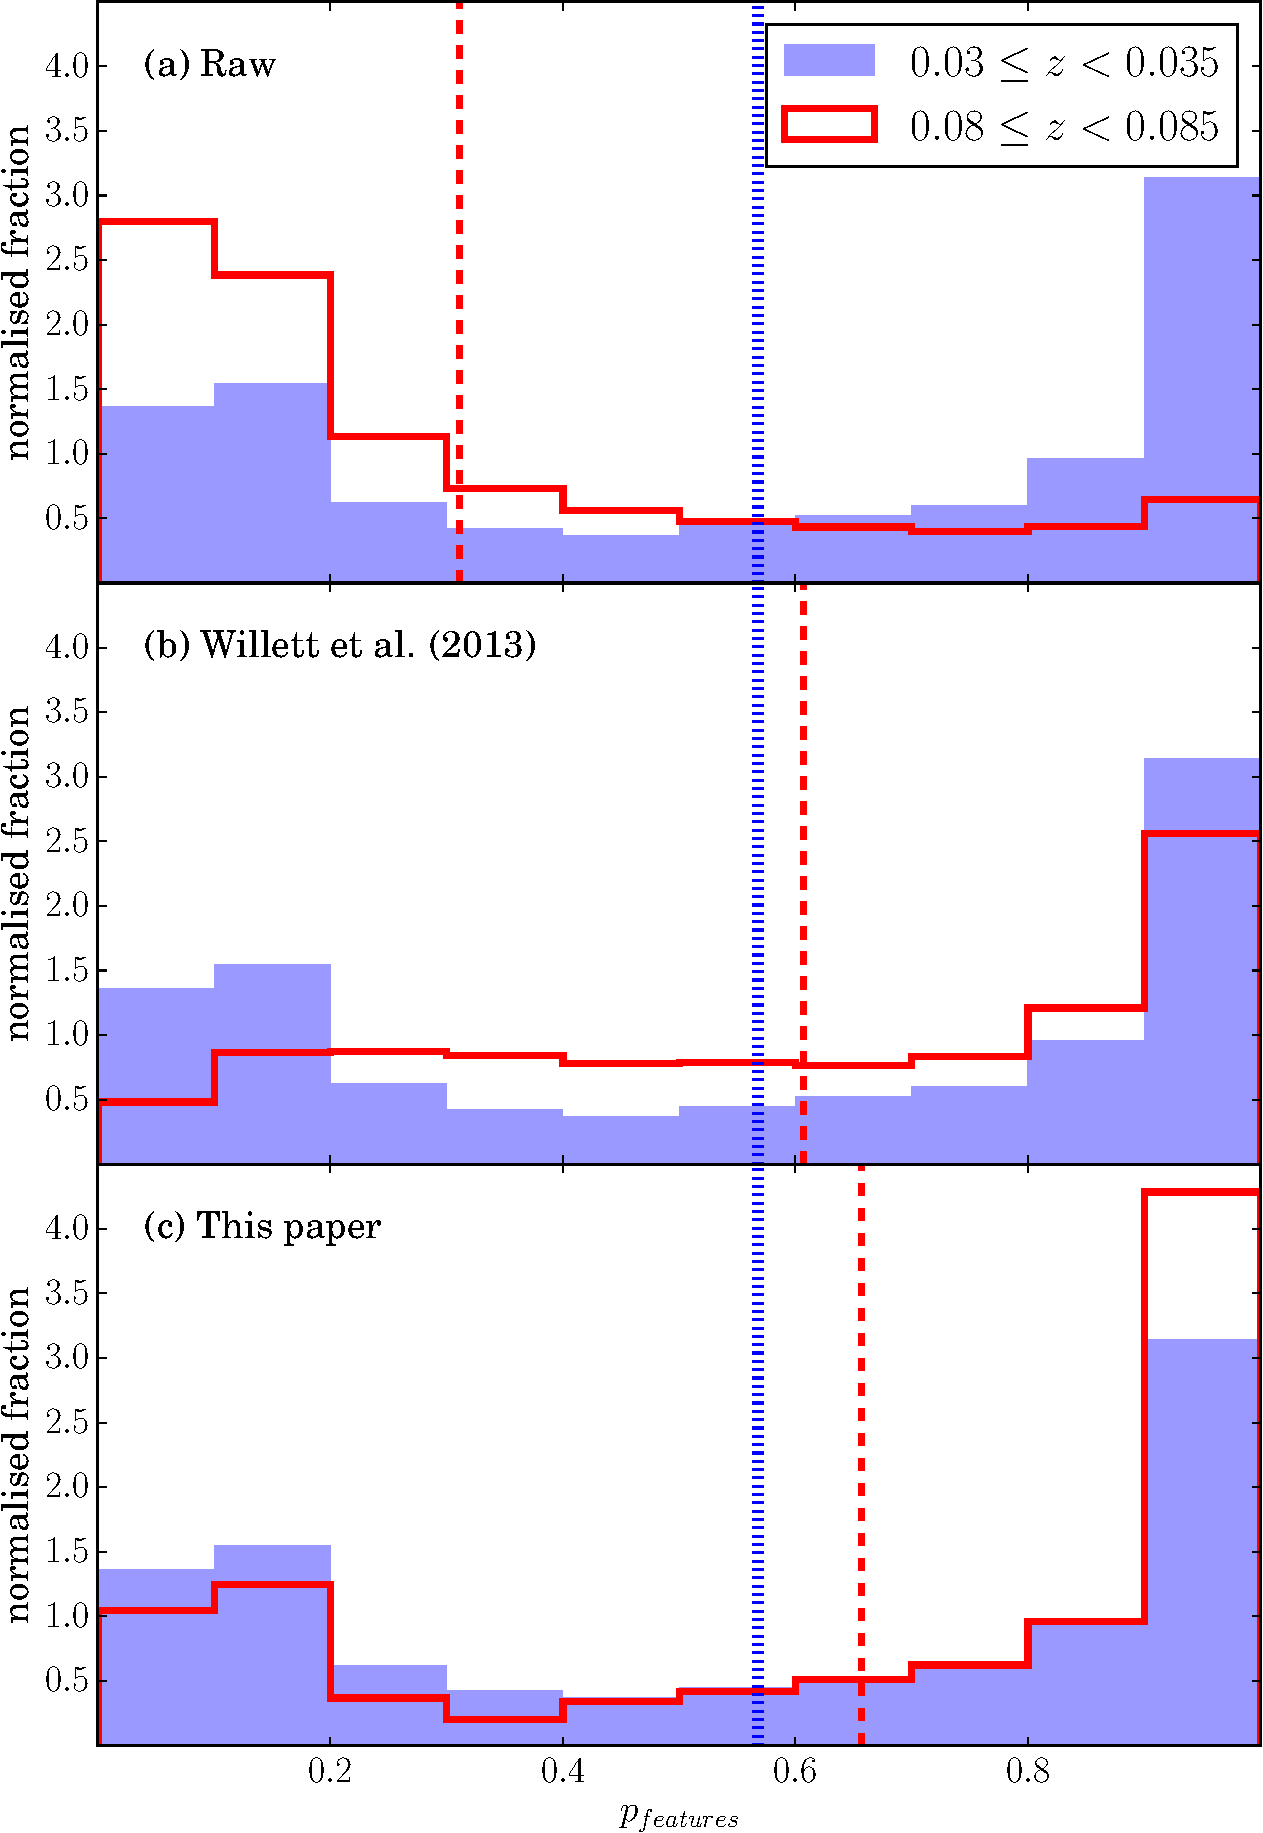
\includegraphics[width=0.45\textwidth]{Images/Bias/Biases/comparison_histogram-crop.pdf}

        \caption{Histograms of vote distributions for the question of whether galaxies are `smooth' or contain `features' in GZ2. The filled blue histogram shows a low redshift sample and the red line indicates a high redshift sample. Both samples are from the \textit{luminosity-limited sample}. The dotted blue line indicates the mean $p_{features}$ value from the low-redshift sample and dashed red line shows the same value for the higher redshift sample.}

        \label{fig:vote_histograms}

\end{figure}
%------------------------------------------------------------------------------------
\subsection{Previous attempt to correct for redshift bias}
\label{sec:previous_method}

The previous debiasing procedure applied to both GZ1 and GZ2 has focused on adjusting the vote fractions of the galaxy samples by fixing the mean vote fractions as a function of redshift. The method was first proposed in \cite{Bamford_09}, and updated for GZ2 in W13. The method successfully adjusts the mean vote fraction for questions with two dominant answers, as can be seen from the vertical lines in Fig.~\ref{fig:vote_histograms}b- the red dashed line of the high-redshift sample is much closer to the blue vertical line from the low-redshift sample than in the raw vote distributions (Fig.~\ref{fig:vote_histograms}a).

However, this technique has two limitations that make it unsuitable if we want to divide a galaxy sample in to different morphology subsets.  The first issue is that adjustment of the mean vote fraction does not necessarily lead to correct adjustment of individual vote fractions, an effect that can be seen in the overall distributions of Fig.~\ref{fig:vote_histograms}b.  Although the mean fractions for the high-redshift sample have been correctly adjusted to approximately match the low-redshift sample, the overall distributions are not necessarily correctly adjusted. Although the mean values match, we see that there is an excess of debiased votes in the middle of the distribution, and fewer votes for the tails of the distribution at $p \approx 0$ and $p \approx 1$. This effect is important if we wish to divide our sample into different subsets by morphological type- as the shape of the histograms is not consistent with redshift, the fraction of galaxies with $p_{features}$ greater than a given threshold can also vary with redshift.

As described in section \ref{sec:gz_morphologies}, GZ2 utilises multiple answered questions to obtain more detailed classifications of galaxies than GZ1. In cases where the votes are split between multiple categories, the debiasing method from W13 does not adjust all of the vote fractions correctly. To show this effect, we select a sample of `secure' spiral galaxies with $p_{\textrm{features}} \times p_{\textrm{not edge-on}} \times p_{\textrm{spiral}} > 0.5$, (with the $p$-values corresponding to the debiased values from W13), and plot the mean $p$-values with respect to redshift for each of the arm number responses. A clear trend in $p$ is observed with redshift- the mean $p$ values  increase with redshift for the 1 and 2 spiral arm answers, even after the W13 correction has been applied. For this question, the answers with more spiral arms (3,4 or more than 4 spiral arms) are the `harder to see' features meaning that there are fewer votes for these categories overall at higher redshift. The W13 debiasing method does not adequately adjust the votes with respect to redshift, so we require an alternative method of debiasing to ensure our galaxy samples are complete at all redshifts. We will now describe this new method in \S\ref{sec:new_method}.

\begin{figure}
		\centering

        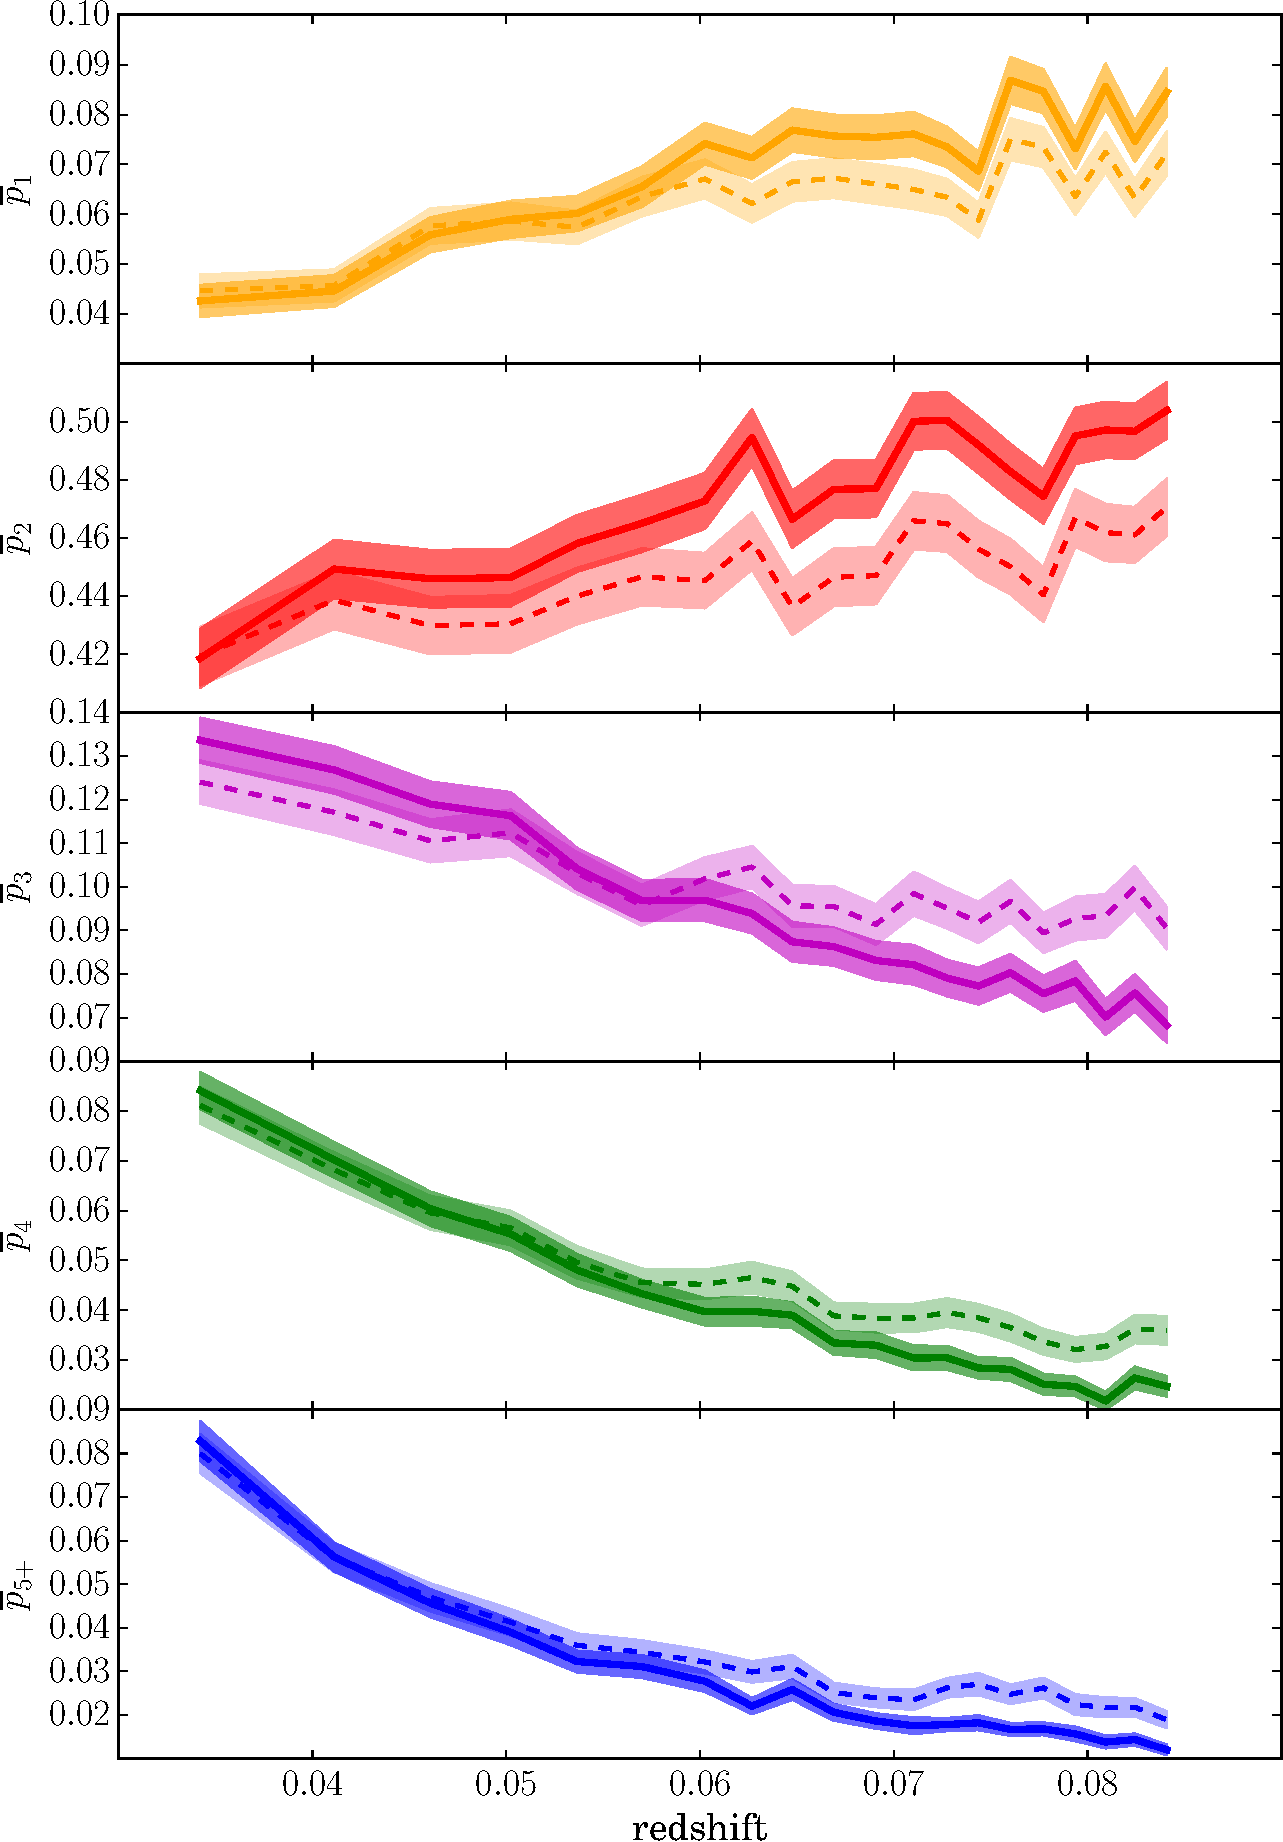
\includegraphics[width=0.45\textwidth]{Images/Bias/Biases/mean_arm_fractions.pdf}

        \caption{Mean value of $p$ for each of the arm number answers. The sample consists of galaxies from the \textit{luminosity-limited sample}, with $p_{features} \times p_{not \, edge-on} \times p_{spiral} > 0.5$ (with $p$-values taken from the W13 debiased catalogue). The solid lines show the mean arm number $p$-values obtained using the raw vote classifications, and the dashed lines indicate the corresponding same quantity obtained using the W13 debiased values. The shaded regions indicate the $1 \sigma$ error on the mean.}

        \label{fig:arm_bias}

\end{figure}
%------------------------------------------------------------------------------------
\subsection{A new method for removing redshift bias}
\label{sec:new_method}

With the limitations described in \S~\ref{sec:previous_method}, we attempt to construct a new method of debiasing the GZ2 data more effectively. This is of particular importance when looking at the question of spiral arm multiplicity (T10 of Fig.~\ref{fig:question_tree}. This is because for a volunteer to have answered the question regarding arm multiplicity, they must have answered a specific answer to three questions previously (that the galaxy has features, is not edge-on and does have spiral arms). Therefore, the number statistics for such galaxies can be very low. When considering a question with low number statistics, such as the spiral arm question, we prefer to use a thresholding technique, rather than using the weighted $p$-values (see \S~\ref{sec:gz_morphologies} for a descriptions of both methods). This is because rarer classes of objects will be affected by noise from the more dominant categories (in this case the two-armed answer). We therefore prefer to divide our galaxy sample in to different sub-samples in order to directly compare them.

Unlike the debiasing method in W13, our new method aims to make the vote distributions themselves as consistent as possible with redshift rather than purely aiming for consistency in the mean vote fraction values. As each galaxy is classified by 40 or more volunteers (W13), we have enough data to model the evolution of the vote distributions as a function of redshift. The theory behind this method is that different classifiers will have different levels of ability to pick out the most detailed features. Thus, as we consider samples at higher redshift, where images have lower signal-to noise, we expect the overall vote fraction trends to also evolve as some classifiers become less able to see the most detailed features. We aim to model this redshift bias by modelling the vote fraction distributions as a function of redshift, and correcting the higher redshift vote distributions to be as similar as possible to equivalent vote distributions at low redshift. 

To do this, we first define samples of galaxies with $p>0.5$ for each of the questions in turn. The entire galaxy sample is then binned in terms of the intrinsic galaxy properties of size and luminosity, and each of these bins is divided in to redshift slices. We then attempt to model the vote distributions for each of the bins with respect to redshift, matching their distributions to those at low redshift. This means that if a threshold is made, the fraction of galaxies with a given feature remains constant, and the sample is composed of the galaxies that are most likely to have that particular feature.  It must also be noted that such a method could still be limited by number statistics at higher redshift. In the case that a rare feature's $p$-value drops to 0 at higher redshift, we can not `add-in' votes- it is only possible to debias the galaxies with $p>0$, which may change significantly with redshift in the rarest categories where the vote fractions are lowest.
%------------------------------------------------------------------------------------
\subsubsection{Sample selection for each question}
\label{sec:sample_selection_per_question}

As GZ2 morphologies are classified with a decision tree (see section \ref{sec:gz_morphologies}), not all of the questions were answered by each of the volunteers. Using the example of spiral arm number, for an individual classifier to have answered the question regarding arm number, they would also have needed to answer that the galaxy they saw had features, was not edge-on and had spiral arms. To avoid `noise' introduced by incorrectly classified galaxies, clean galaxy samples are defined with $p > 0.5$. For the first question, this corresponds to all of the galaxies, as each classifier answered that particular question for each galaxy. However, when questions further down the tree are considered, this is not the case. The equiavalent $p>0.5$ for the spiral arm question would only include the galaxies with $p_{\textrm{features}} \times p_{\textrm{not edge-on}} \times p_{\textrm{spiral}} > 0.5$. 

For each of the questions in turn, we define a sample of galaxies with which we will apply the new debiasing procedure. These samples are defined using a cut of $p>0.5$ (corresponding to $p_{\textrm{features}} \times p_{\textrm{not edge-on}} \times p_{\textrm{spiral}} > 0.5$ for the spiral arm question for example). A further cut of $N \geq 5$ (where $N$ is the number of classifications) is also imposed to ensure that each galaxy has been classified by a significant number of people to reduce the effects of noise. In this case, the $p$-values must be the debiased vote values, to ensure each sample is as complete as possible (see \S~\ref{sec:biases}) as we look at each question. This means that the order in which the questions are debiased is important- to define a sample for the debiasing of a particular question, all questions further up the question tree must have been debiased beforehand.
%------------------------------------------------------------------------------------
\subsubsection{Binning the data}
\label{sec:binning}

It is expected that galaxy morphological properties, such as the presence of a particular feature, will depend on intrinsic galaxy properties.  For example, larger, brighter galaxies may be easier to classify over a wider redshift range. Conversely, fainter galaxies may show stronger features, as the fraction of spiral galaxies is higher for galaxies with lower absolute magnitudes \rh{cite???}. To account for these possible variations, we voronoi tesselate the data in terms of $M_r$ and $\log(R_{50})$ for each answer in turn using the \texttt{voronoi\_2d\_binning} package from \cite{Cappellari_03}, meaning that each of the bins should contain an aproximately equal number of galaxies.  An example of a voronoi tesselation of our sample is shown in Fig.~\ref{fig:voronoi_bins}. When voronoi tesselating the data for each of the answers, only the galaxies with $p>0$ are included, meaning that the `signal' of galaxies is evened out over all of the voronoi bins. We aim to have $\sim 30$ voronoi bins for each of the questions, so the bin signal for each of the voronoi bins is given as $N_{gal}/30$, where $N_{gal}$ is the number of galaxies with $p>0$.  

\begin{figure}
		\centering

        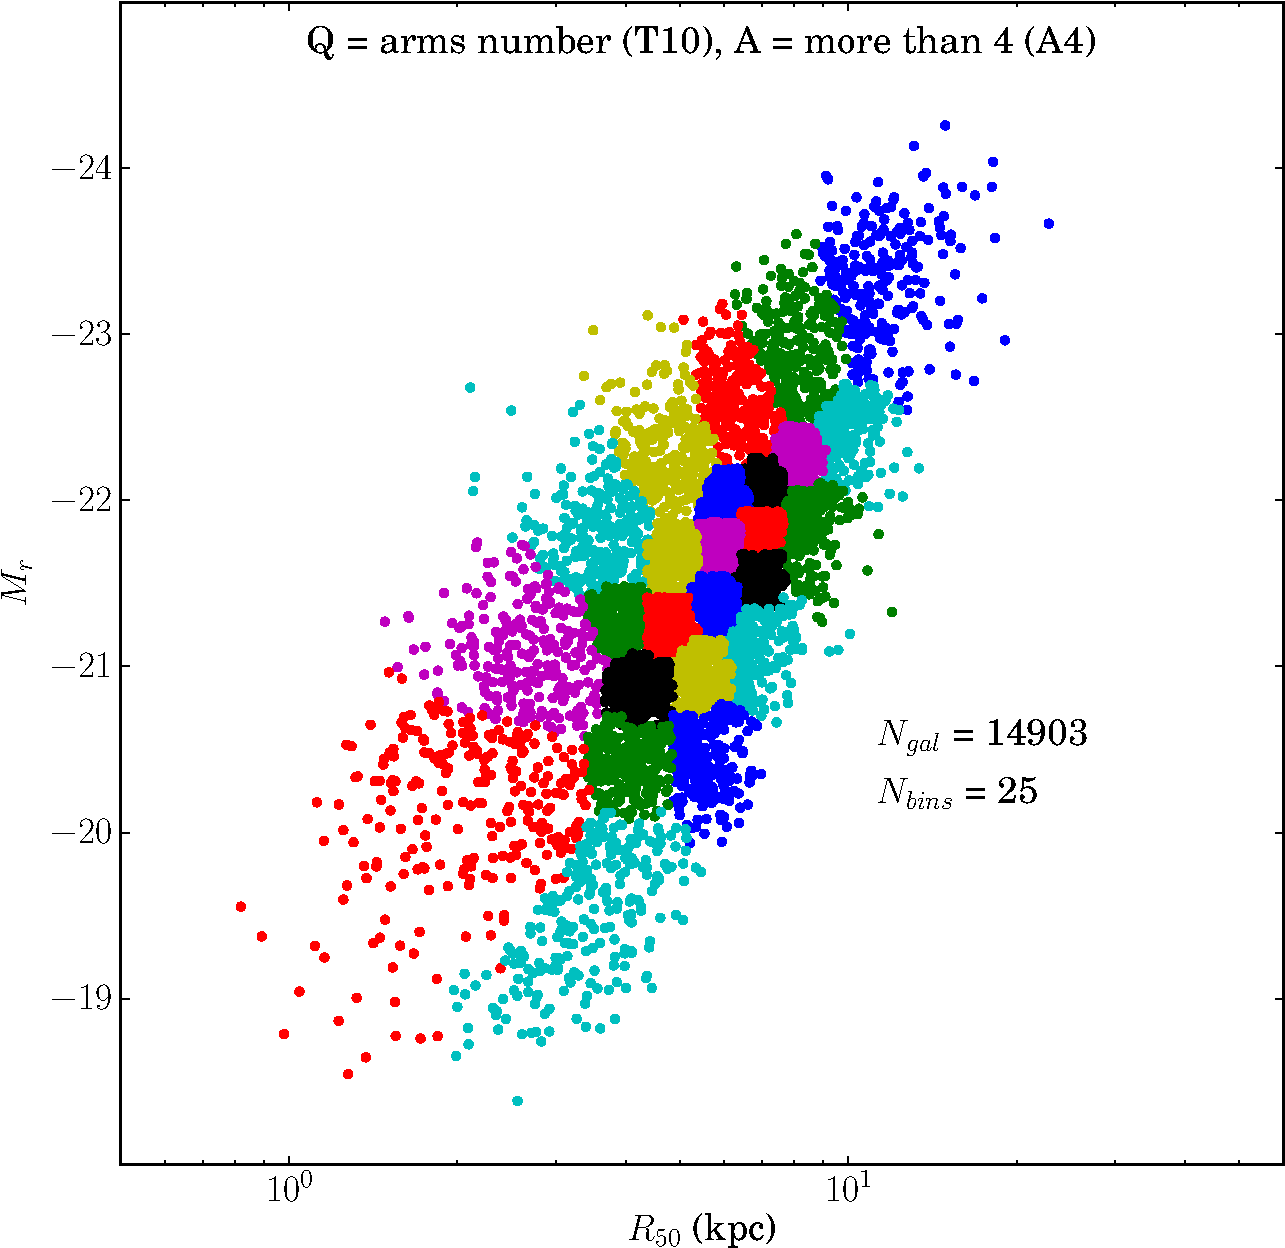
\includegraphics[width=0.45\textwidth]{Images/Bias/Debiasing/voronoi_bins.pdf}

        \caption{Distribution of the voronoi bins in terms of $R_{50}$ and $M_r$ for the spiral arm number question and the more than 4 spiral arms answer. Each of the voronoi bins is further divided in to redshift bins, each with $\geq 50$ galaxies.}

        \label{fig:voronoi_bins}

\end{figure}

After voronoi binning the data in terms of their intrinsic properties of size and brightness, we further divide the sample in to redshift bins, to allow us to look in to how the vote distributions change with redshift. To ensure that there is a good signal in each of the redshift bins, we divide each of the voronoi bins in to redshift bins, each containing containing $\geq 50$ galaxies. This binned data is used for the debiasing methods described in \S~\ref{sec:debiasing}.
%------------------------------------------------------------------------------------
\subsubsection{Modelling redshift bias}
\label{sec:debiasing}

For each of the possible responses to each question, a method is applied to correct for the redshift bias in the sample. The first stage is to select a sample as described in section \ref{sec:sample_selection_per_question} as a reference, and to bin the data using the method described in section \ref{sec:binning}. As described in section \ref{sec:new_method}, we aim to make the vote distributions for each answer consistent with redshift. The two methods that we employ to achieve this are described below. 

The first method we utilise remove redshift bias simply matches the shapes of the histograms on a `bin-by-bin' basis. The vote fractions for the given answer are ranked from lowest $p$-value to highest $p$-value, and a cumulative histogram is plotted. The cumulative distribution for the lowest redshift sample in a given voronoi bin is used as a reference for how the shape of the histogram would look if it were viewed at low redshift. An example of this method is shown in Fig.~\ref{fig:histogram_matching}, in which the `features or disk' answer to the `smooth or features' question is considered. For each of the higher redshift samples in that same voronoi bin, the ranked votes are matched to those at lower redshift. This means that applying a threshold gives the same fraction of galaxies above that given threshold in both the high and low redshift bins, with the galaxies most likely to have a given feature making up the population of galaxies above that threshold. 

\begin{figure}
		\centering

        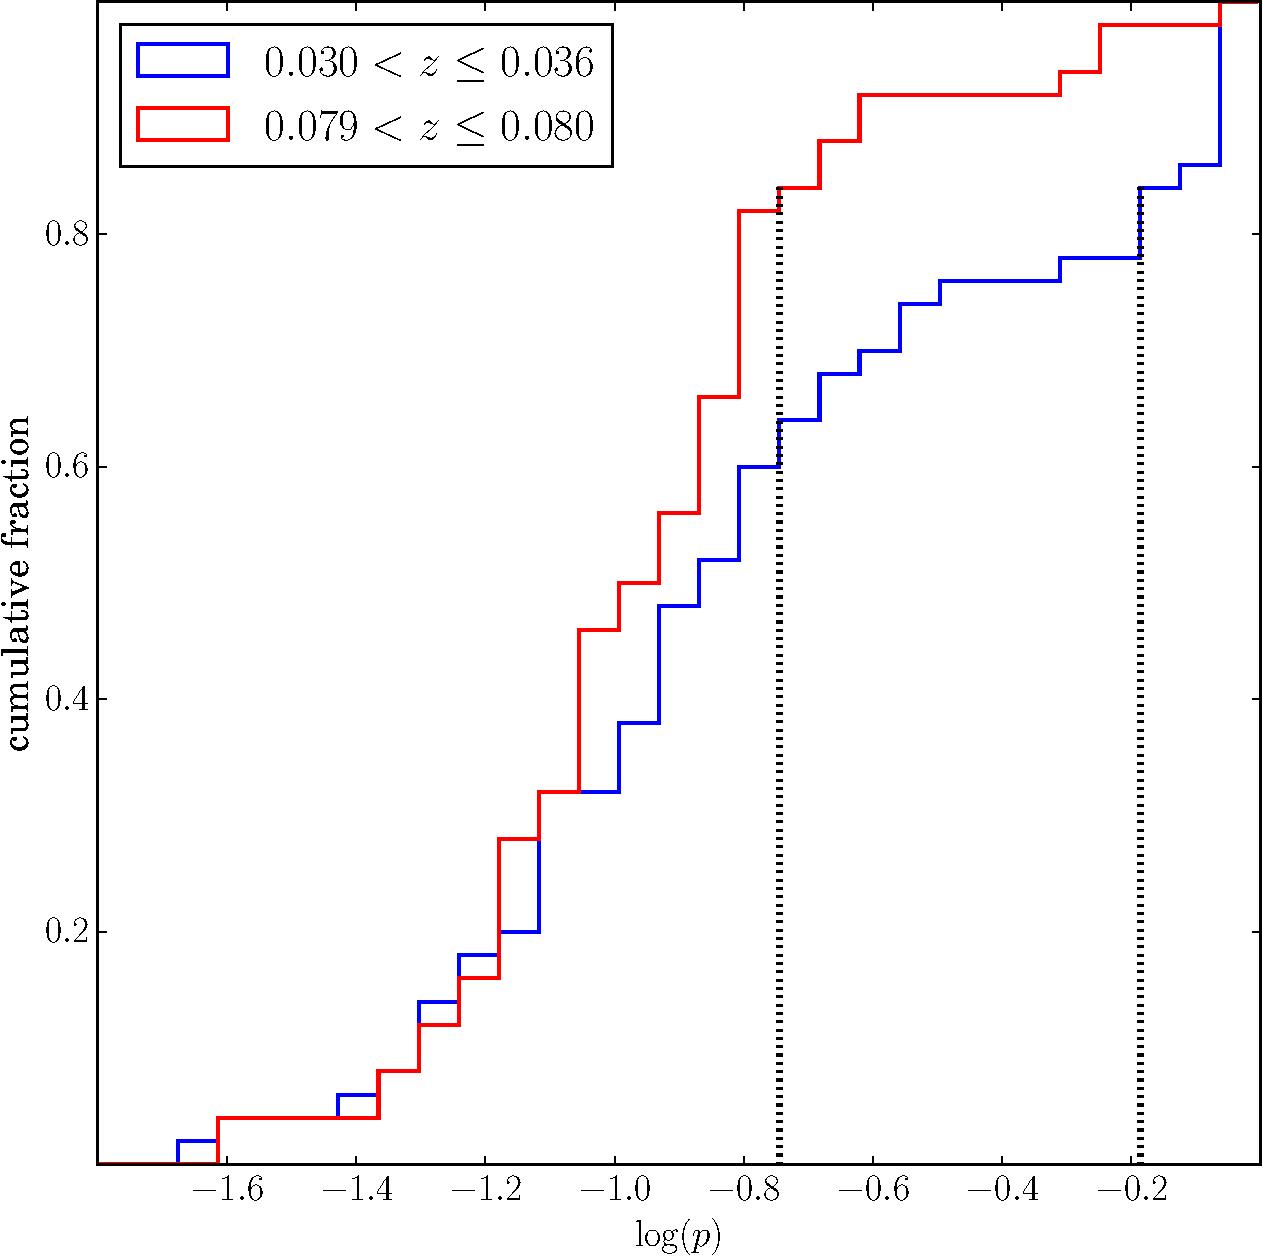
\includegraphics[width=0.45\textwidth]{Images/Bias/Debiasing/histogram_matching.pdf}

        \caption{An example of vote distributions for an example voronoi bin for the `features or disk' answer to the `smooth or features' question. Each of the galaxies in the high-redshift bin (red line) is matched to its closest equivalent low-redshift galaxy (blue line) in terms of cumulative fraction. The dashed lines indicate the `matched' values for an example galaxy with $\log(p) \approx 0.8$, and an equivalent low-redshift value of $\log(p) \approx 0.2$(corresponding to $p_{raw}=0.18$ and $p_{debiased}=0.65$).}

        \label{fig:histogram_matching}

\end{figure}

\begin{figure*}
		\centering

        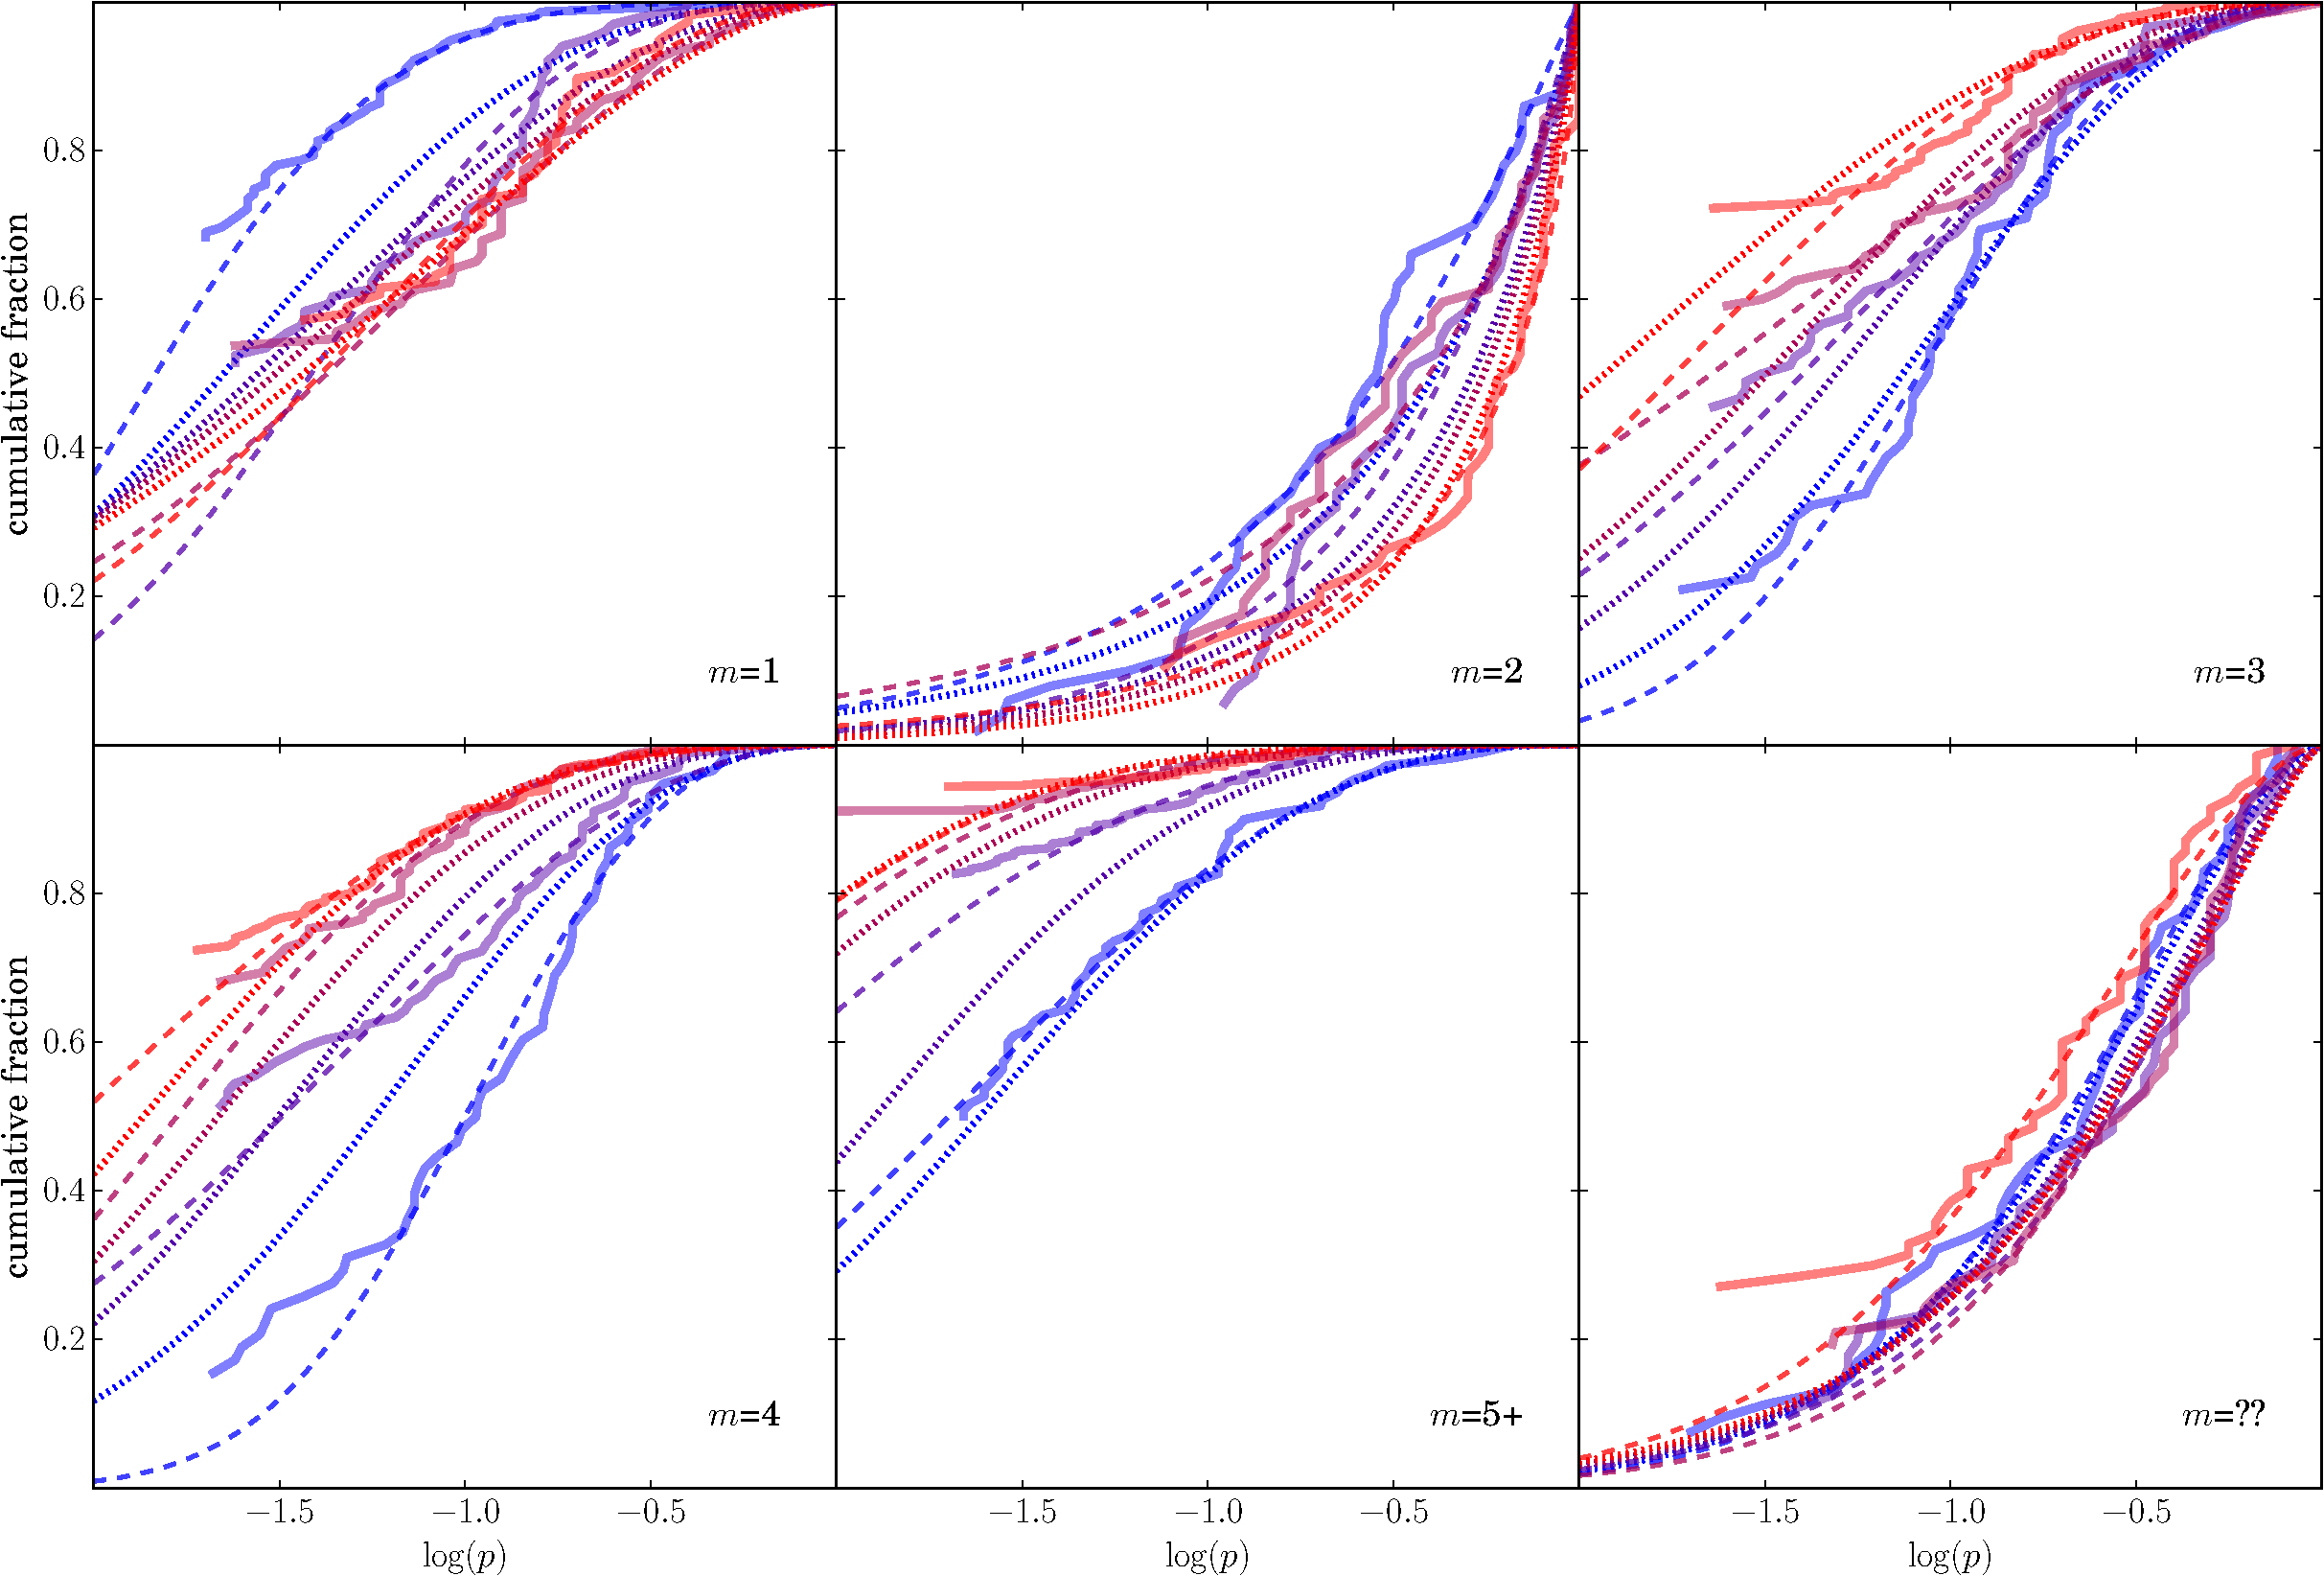
\includegraphics[width=0.975\textwidth]{Images/Bias/Debiasing/vbin_fit.pdf}

        \caption{An example of a single voronoi bin fit for the \textit{arm number} question. The red line indicates the highest redshift bin, and the blue line indicates the lowest redshift bin. The solid lines indicate the raw $p$ histograms, and the dashed lines show the best fit function to each of them. The dotted lines show the corresponding approximation from the continous fit to the $k$ and $c$ values.}

        \label{fig:function_fit}

\end{figure*}

The main strength of this method is that any vote distribution can be modelled in this way, irrespective of the overall shape. However, a potential weakness is that noise can be introduced due to the discretisation of the data. This can cause issues when the number statistics are low in questions where the sample size is severely reduced because of the number of questions that have come before it (see \S~\ref{sec:sample_selection_per_question}), which means that the bins have to span a wide redshift range to achieve a `good' signal of $\geq50$ galaxies per bin. One potential solution would be to bin the data more finely. However, there is no `ideal' solution to this problem- fewer galaxies in each bin would mean that the redshift range that each bin occupies would be smaller, but the overall noise in terms of the range of galaxy morphologies within each bin would increase. 

To attempt to remove the discrete nature of the correction in the `bin-by-bin' method, an alternative approach is proposed that attempts to model vote distributions with functions. For each of the redshift bins, we plot a cumulative histogram of $\log(p)$ against cumulative fraction. An example of some of these cumulative histograms are plotted as the solid lines in Fig.~\ref{fig:function_fit}. It can be seen that there is a clear evolution in the distributions with redshift. This effect is most prominent in the $m=4$ and $m=5+$ responses, where the overall distributions shift so that there are fewer votes for higher $p$-values. To attempt to correct for this bias, each of the cumulative histograms can be modelled with a function, and the parameters of the function can be modelled in terms of redshift($z$), galaxy size ($R_{50}$) and intrinsic brightness ($M_r$). An exponential function of the following form is used to model the distributions:

\begin{equation}
f(p) = e^{kp^{c}}
\end{equation}

where $k$ and $c$ parameterise the shape of each of the curves. Best-fit $k$ and $c$ values are found for each of the bins using the \texttt{scipy.optimize.minimize} package (\rh{cite?}), indicated by the dashed lines in Fig.~\ref{fig:function_fit}. When fitting the data, the data is sampled evenly in $\log(p)$ to avoid the fit being weighted to the most steep parts of the curves. 

After finding $k$ and $c$ for each of the bins, we attempt to quantify how these parameters change with respect to $M_r$, $\log(R_{50})$ and $z$. Firstly, we apply a $2\sigma$ clipping to $k$ and $c$ to remove any fits that where $k$ or $c$ values have been found. The data is then fitted using a continuous function of the following form:

\begin{equation}
\begin{split}
A_{fit}(M_r,R_{50},z) = & A_0 + A_M(f_M(-M_r)) +\\
						& A_R(f_R(\log({R_{50}}))) + A_z(f_z(z))
\end{split}
\end{equation}

where $A$ corresponds to either $k$ or $c$ and $f_M$, $f_R$ and $f_z$ are functions that can be either logarithmic ($\log(x)$), linear ($x$) or exponential ($e^x$) (where x is either $-M_r$, $\log(R_{50})$ or $z$). The values $A_0$, $A_M$, $A_R$ and $A_z$ are constants that parameterise the shape of the fit with respect to each of the terms. When fitting the data, $M_r$, $\log(R_{50})$ and $z$ correspond to their respective mean values calculated using all of the galaxies in that bin. The best combination of functions is chosen by calculating $A_0$, $A_M$, $A_R$ and $A_z$ for each combination of $f_M$, $f_R$ and $f_z$ using the \texttt{scipy.optimize.curve\_fit} package, and selecting the function that has the lowest square residual to find $k_{fit}$ and $c_{fit}$ continuous functions. We then clip any values with a $>2\sigma$ residual to this fit and re-fit the data to find a final functional form for $k$ and $c$ with respect to $M_r$, $R_{50}$ and $z$. Some $k_{fit}$ and $c_{fit}$ values at the $M_r$, $R_{50}$ and $z$ values of the bins for the \textit{spiral arm number} question are shown by the dotted lines of Fig.~\ref{fig:function_fit}.

\rh{*Do we need some kind of plot to show how k and c have been fitted here?}

Limits are also applied to $k$ and $c$ to avoid unphysical fits at extreme values of $M_R$, $R_{50}$ and $z$. The range of $k$ and $c$ is therefore set by the upper and lower limits of all of the fit $k$ and $c$ values within the $2\sigma$ clipping.

After finding a functional form for $k$ and $c$ with respect to $M_r$, $\log(R_{50})$ and $z$, each of the galaxies in the sample is debiased to find equivalent values at low redshift. To do this for an individual galaxy, the shape of its cumulative histogram is estimated using $k_{fit}(M_r,R_{50},z)$ and $c_{fit}(M_r,R_{50},z)$, where $M_r$,$R_{50}$ and $z$ are the properties for that particular galaxy. The equivalent function at $z=0.03$ (the low redshift limit of our \textit{luminosity-limited sample}) is also found for a galaxy with the same size and luminosity, using $k_{fit}(M_r,R_{50},0.03)$ and $c_{fit}(M_r,R_{50},0.03)$. The corresponding $p$-value for a given cumulative fraction is read off from the low redshift distribution in a similar way as in the bin-by-bin method, but this time using the fitted curves rather than the raw histograms. This is repeated for each of the galaxies in the sample to generate a set of debiased values for the \textit{full sample} of galaxies.

As mentioned previously, function fitting does not suffer from the defects introduced by the discretisation of the data. However, it does introduce its own biases, as an assumption is made that the cumulative histograms can all be well-fit by a continuous function. This may not always be the case, so we must consider which of the above methods does the best overall job of removing redshift bias. 

To decide which of the two methods should be preferred, the \textit{luminosity-limited sample} is used, as this sample is free from any redshift bias. A low redshift slice of this data ($0.03 \leq z < 0.035$) is used as reference. The square residual of the $p$-value debiased distributions in 10 redshift slices of the total \textit{luminosity-limited sample} is calculated for the debiased values from both methods. The method that has the lowest overall square residual is taken as the preferred method, and those are the dabiased values used as the $p$-values for that response.
%------------------------------------------------------------------------------------
\subsubsection{Results from the new debiasing method}
\label{sec:debiasing_results}

\begin{figure*}
		\centering

        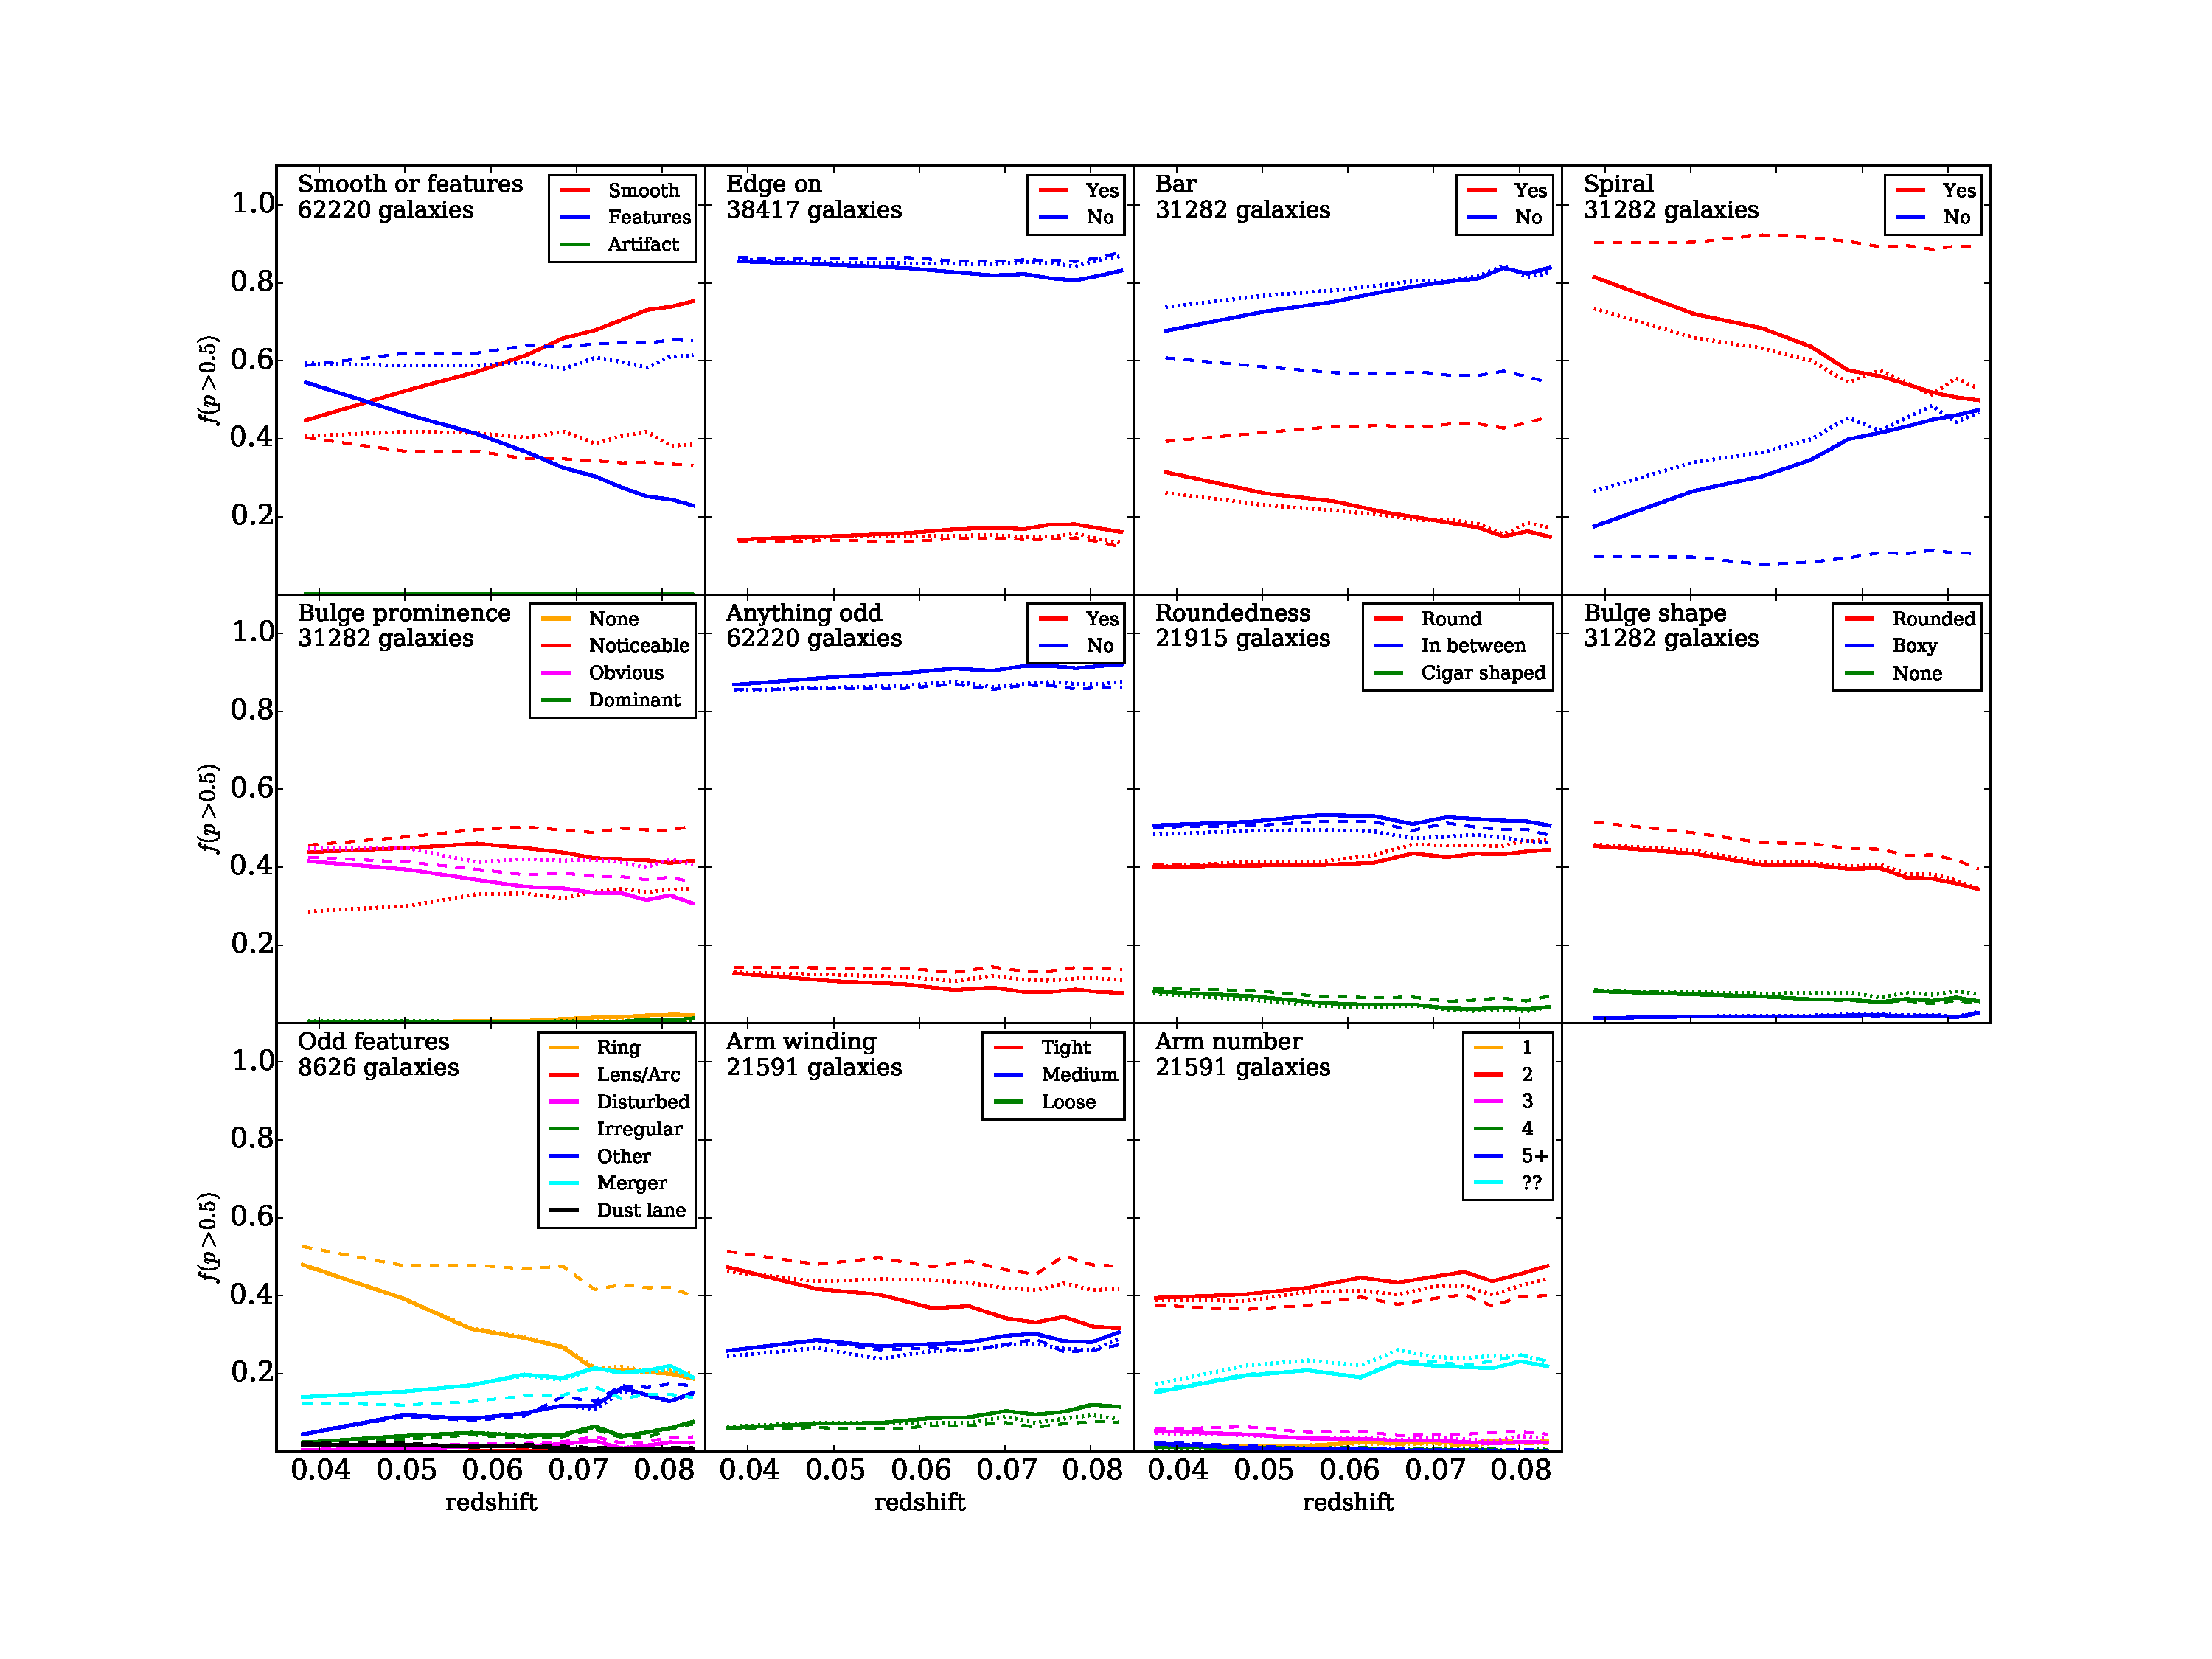
\includegraphics[width=0.975\textwidth]{Images/Bias/Debiasing/all_thresholds.pdf}

        \caption{Number of galaxies with $p>0.5$ for each of the questions debiased using the method described in section \ref{sec:new_method}. The solid lines indicate the raw vote fractions and the dashed lines indicate the debiased vote fractions. The dotted lines indicate the same fractions using the W13 debiasing method. The total sample here is composed of galaxies in the \textit{luminosity-limited sample} with $p>0.5$ (as described in \S~\ref{sec:sample_selection_per_question}).}

        \label{fig:all_thresholds}

\end{figure*}

\begin{figure*}
		\centering

        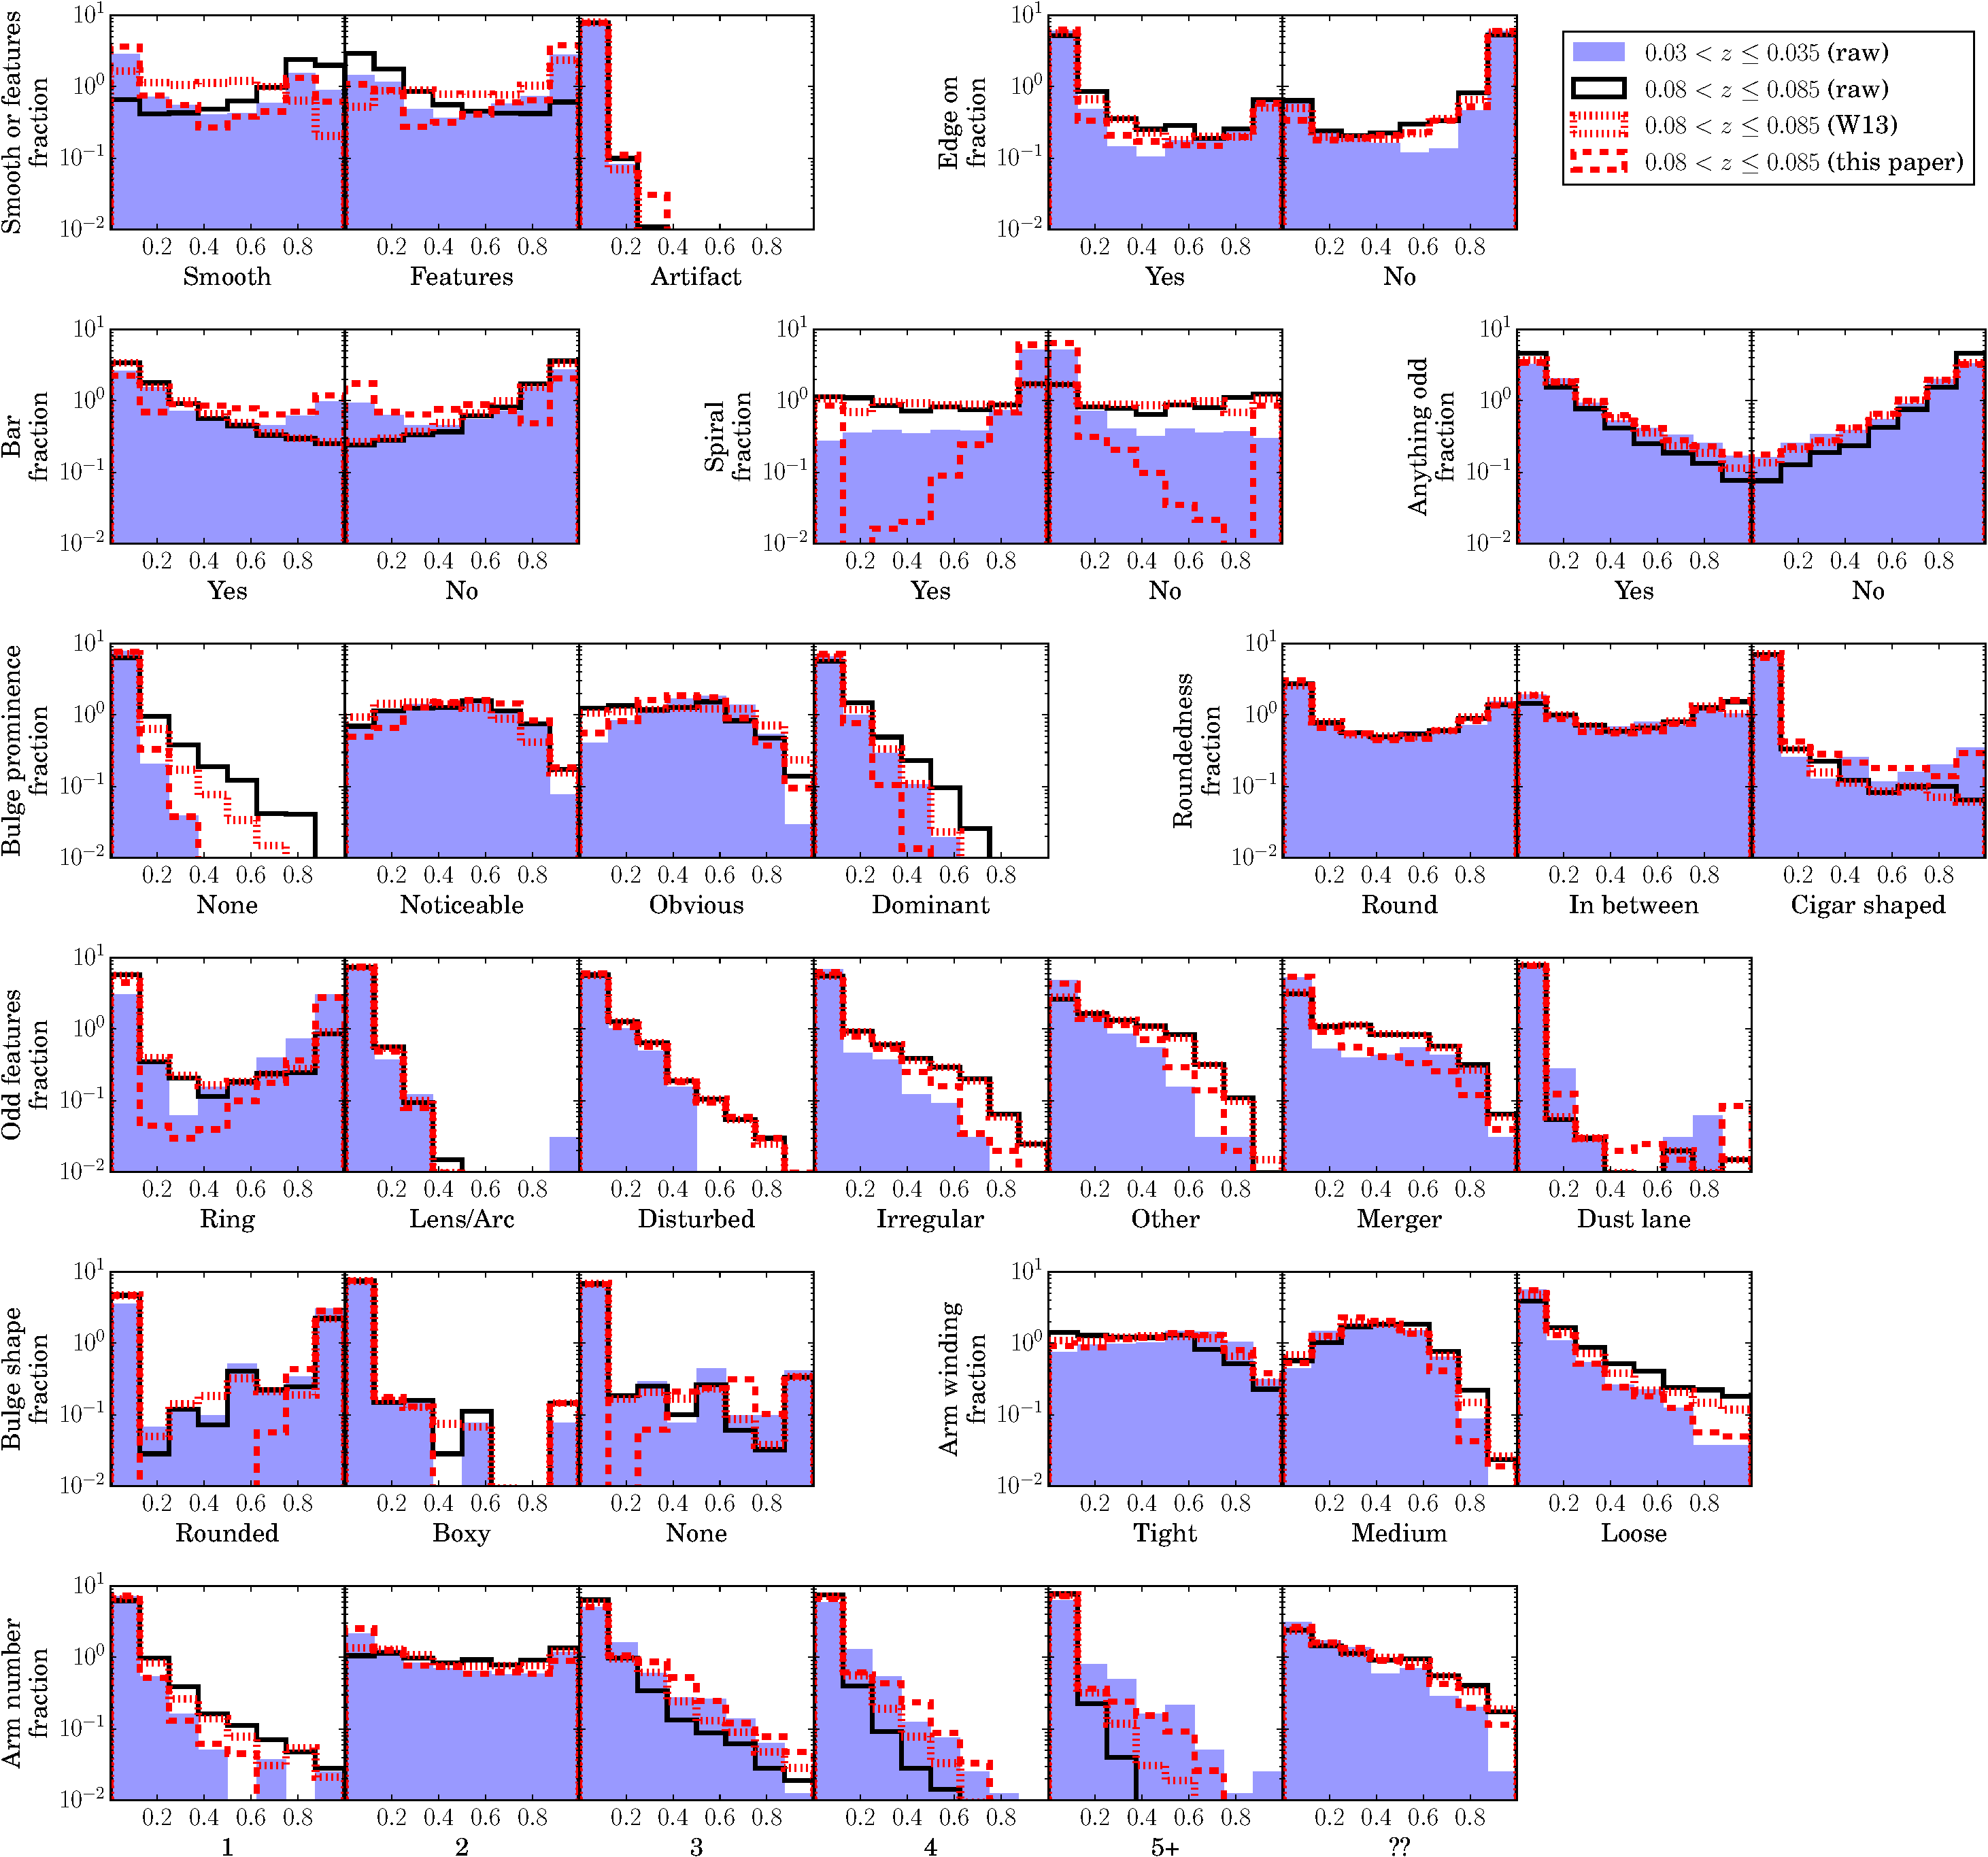
\includegraphics[width=0.975\textwidth]{Images/Bias/Debiasing/all_histograms.pdf}

        \caption{Vote distribution histograms for each of the answers in the GZ2 question tree. The blue filled histogram shows the distribution for a low redshift $0.03< z \leq 0.035$ sample, which should have minimal redshift-dependent bias. The black solid, red dotted and red dashed histograms show the higher redshift $0.08 < z \leq 0.085$ distribution of the raw, W13 debiased and debiased data from this paper respectively. Both the low and higher redshift distributions are drawn from galaxies with $p>0.5$ (as described in \S~\ref{sec:sample_selection_per_question}) from the \textit{luminosity-limited sample}.}

        \label{fig:all_histograms}

\end{figure*}

As described in \S~\ref{sec:new_method}, the new method aims to keep the number of galaxies above a given threshold constant with redshift, rather than simply correcting the mean overall $p$-values with redshift. To test how successful the new debiasing method is at defining populations of galaxies above a given threshold with redshift, the fraction of galaxies with $p>0.5$ for each of the questions is plotted in Fig.~\ref{fig:all_thresholds}. It can be seen that in most cases, the new debiasing method does keep the fraction of the population with $p>0.5$ constant with redshift, as expected. This effect is most evident when looking at the \textit{spiral} question, in the top right-hand side of Fig.~\ref{fig:all_thresholds}. It can be seen that the original debiasing method does not adequately remove redshift bias, with fewer galaxies exhibiting spiral structure at higher redshift. However, this method does keep this fraction approximately constant with redshift, which means the spiral sample will be complete if we wish to use a thresholding technique to separate galaxies in to samples of galaxies with spiral structure and galaxies which do not. 

It must also be noted that Fig.~\ref{fig:all_thresholds} only shows the specific example of the threshold of $p>0.5$. This does not give any insight into the overall $p$-value distribution. Therefore, overall distributions are compared for two redshift slices in Fig.~\ref{fig:all_histograms}. 

\rh{Can we include some RMS values to show what's going on? Particularly point out that we're much better for our question branch?}


%------------------------------------------------------------------------------------
%%%%%%%%%%%%%%%%%%%%%%%%%%%%%%%%%%%%%%%%%%%%%%%%%%%%%%%%%%%%%%%%%%%%%%%%%%%%%%%%%%%%%
%------------------------------------------------------------------------------------
\section{Properties of spiral galaxies with respect to arm number}
\label{sec:results}

Spiral galaxies make up as many as two-thirds of the galaxies in the local Universe \citep{Lintott_11,Willett_13}. Most of the star formation in the local Universe occurs in spirals, and in particular is concentrated in the regions of spiral arms \citep{Dobbs_14}. The prominence of spiral structure itself means that understanding the physical processes responsible for spiral structure is vital in understanding how galaxies evolved, and how star-formation itself occurs and evolves.

Depite how prevelant spiral structure is on the local Universe, finding a complete picture as to how it forms is still elusive. One of the key reasons why this is the case is because spiral structure can take many varied appearances. Classifying spiral galaxies is generally done using either a Hubble-type classification scheme \citep{Hubble_26} or an Elmegreen-type classification scheme \citep{EE_82,EE_87}. However, the Hubble method is based on bulge size and spiral arm pitch angle, which are weakly correlated, indicating that the physical processes that are responsible for those two features are very different \citep{Kennicutt_81,Seigar_98}. The Elmegreen-type classifications scheme instead divides galaxies in to two types depending on the \emph{spiral arm structure} itself, rather than any properties related to the galactic bulge. In particular, the scheme divides galaxies in to `grand design' spirals, with two symmetric spiral arms, and multiple-armed more `flocculent' spirals, with several shorter, less well-defined arms. The distinct advantage to classifying spiral galaxies in this way is that the physical mechanisms that play a role in the formation of these two different types of spiral structure are actually thought to be very different.

`Grand design' spiral structure was initially thought to be due to the presence of a density wave in a galaxy's disk \citep{Lindblad_63,Lin_64}. In the mechanism proposed by \citet{Lin_64}, gas is `shocked' in to star-formation in regions of high density in the disk. However, this mechanism is no longer favoured, as there is no evidence for the enhancement of star-formation in `grand design' spiral galaxies compared to many-armed spiral galaxies \citep{Romanishin_85,EE_86}, or any evidence for enhancement in star-formation in the individual arms of such galaxies \citep{Foyle_11,Choi_15}. Instead, it is thought that `grand design' spiral structure may actually be the result of strong bars in spiral galaxies or tidal interactions \citep{Kormendy_79}. Early observational evidence supports the theory that `grand design' structure can be induced via interactions, with two-armed structure being favoured over many-armed structure in high density environments \citep{EE_82,EE_87,Ann_14}, and simulations showing that galaxy-galaxy interactions can lead to the types of grand design spirals seen in the local Universe \citep{Dobbs_10}. 

Unlike two-armed spiral structure, many-armed spiral structure arises readily in simulations without the requirement for a trigger from either a bar instability or a tidal interaction \citep{James_78,Sellwood_84}. Instead such structures arise readily in simulations, but require a cooling of the gas in the disk to be sustained for long periods of time \citep{Carlberg_85}. More recent simulations, taking the disk gravity into account, have shown that `flocculent' structure may actually be a transient feature of spiral galaxies, with spiral arms continually being made and destroyed \citep{Bottema_03,Grand_12b,Baba_09,Baba_13,Donghia_13}, rather than long-lasting persistent structures.

Despite the recent advances in the simulations of these disk galaxies, the picture as to how all of the processes shape spiral galaxies still remains unclear. Grand design spiral galaxies can still reside in low density environments without the presence of a bars  \citep{EE_82}, meaning that they are not purely driven by these processes as described in \citep{Kormendy_79}. Additionally, the timescales of the persistence of spiral structure is still unclear, particularly as older stellar populations viewed in the infra-red show very different structure to the young stellar populations viewed at optical wavelengths \citep{Block_91,Block_94,Thornley_96}. Most recent work on spiral structure have also mainly been focused on simulations of spiral structure; putting observational constraints requires the visual inspection of the spiral arm structure in galaxy disks, so have been restricted to relatively small samples of order $\lesssim$ 2000 galaxies \citep{EE_82,EE_89,Ann_13}. We aim to use GZ2 classifications to measure spiral arm morphology of a much larger sample of SDSS galaxies in the local Universe.
%------------------------------------------------------------------------------------
\subsection{Spiral arms in Galaxy Zoo}
\label{sec:defining_the_sample}

\begin{figure*}
		\centering

        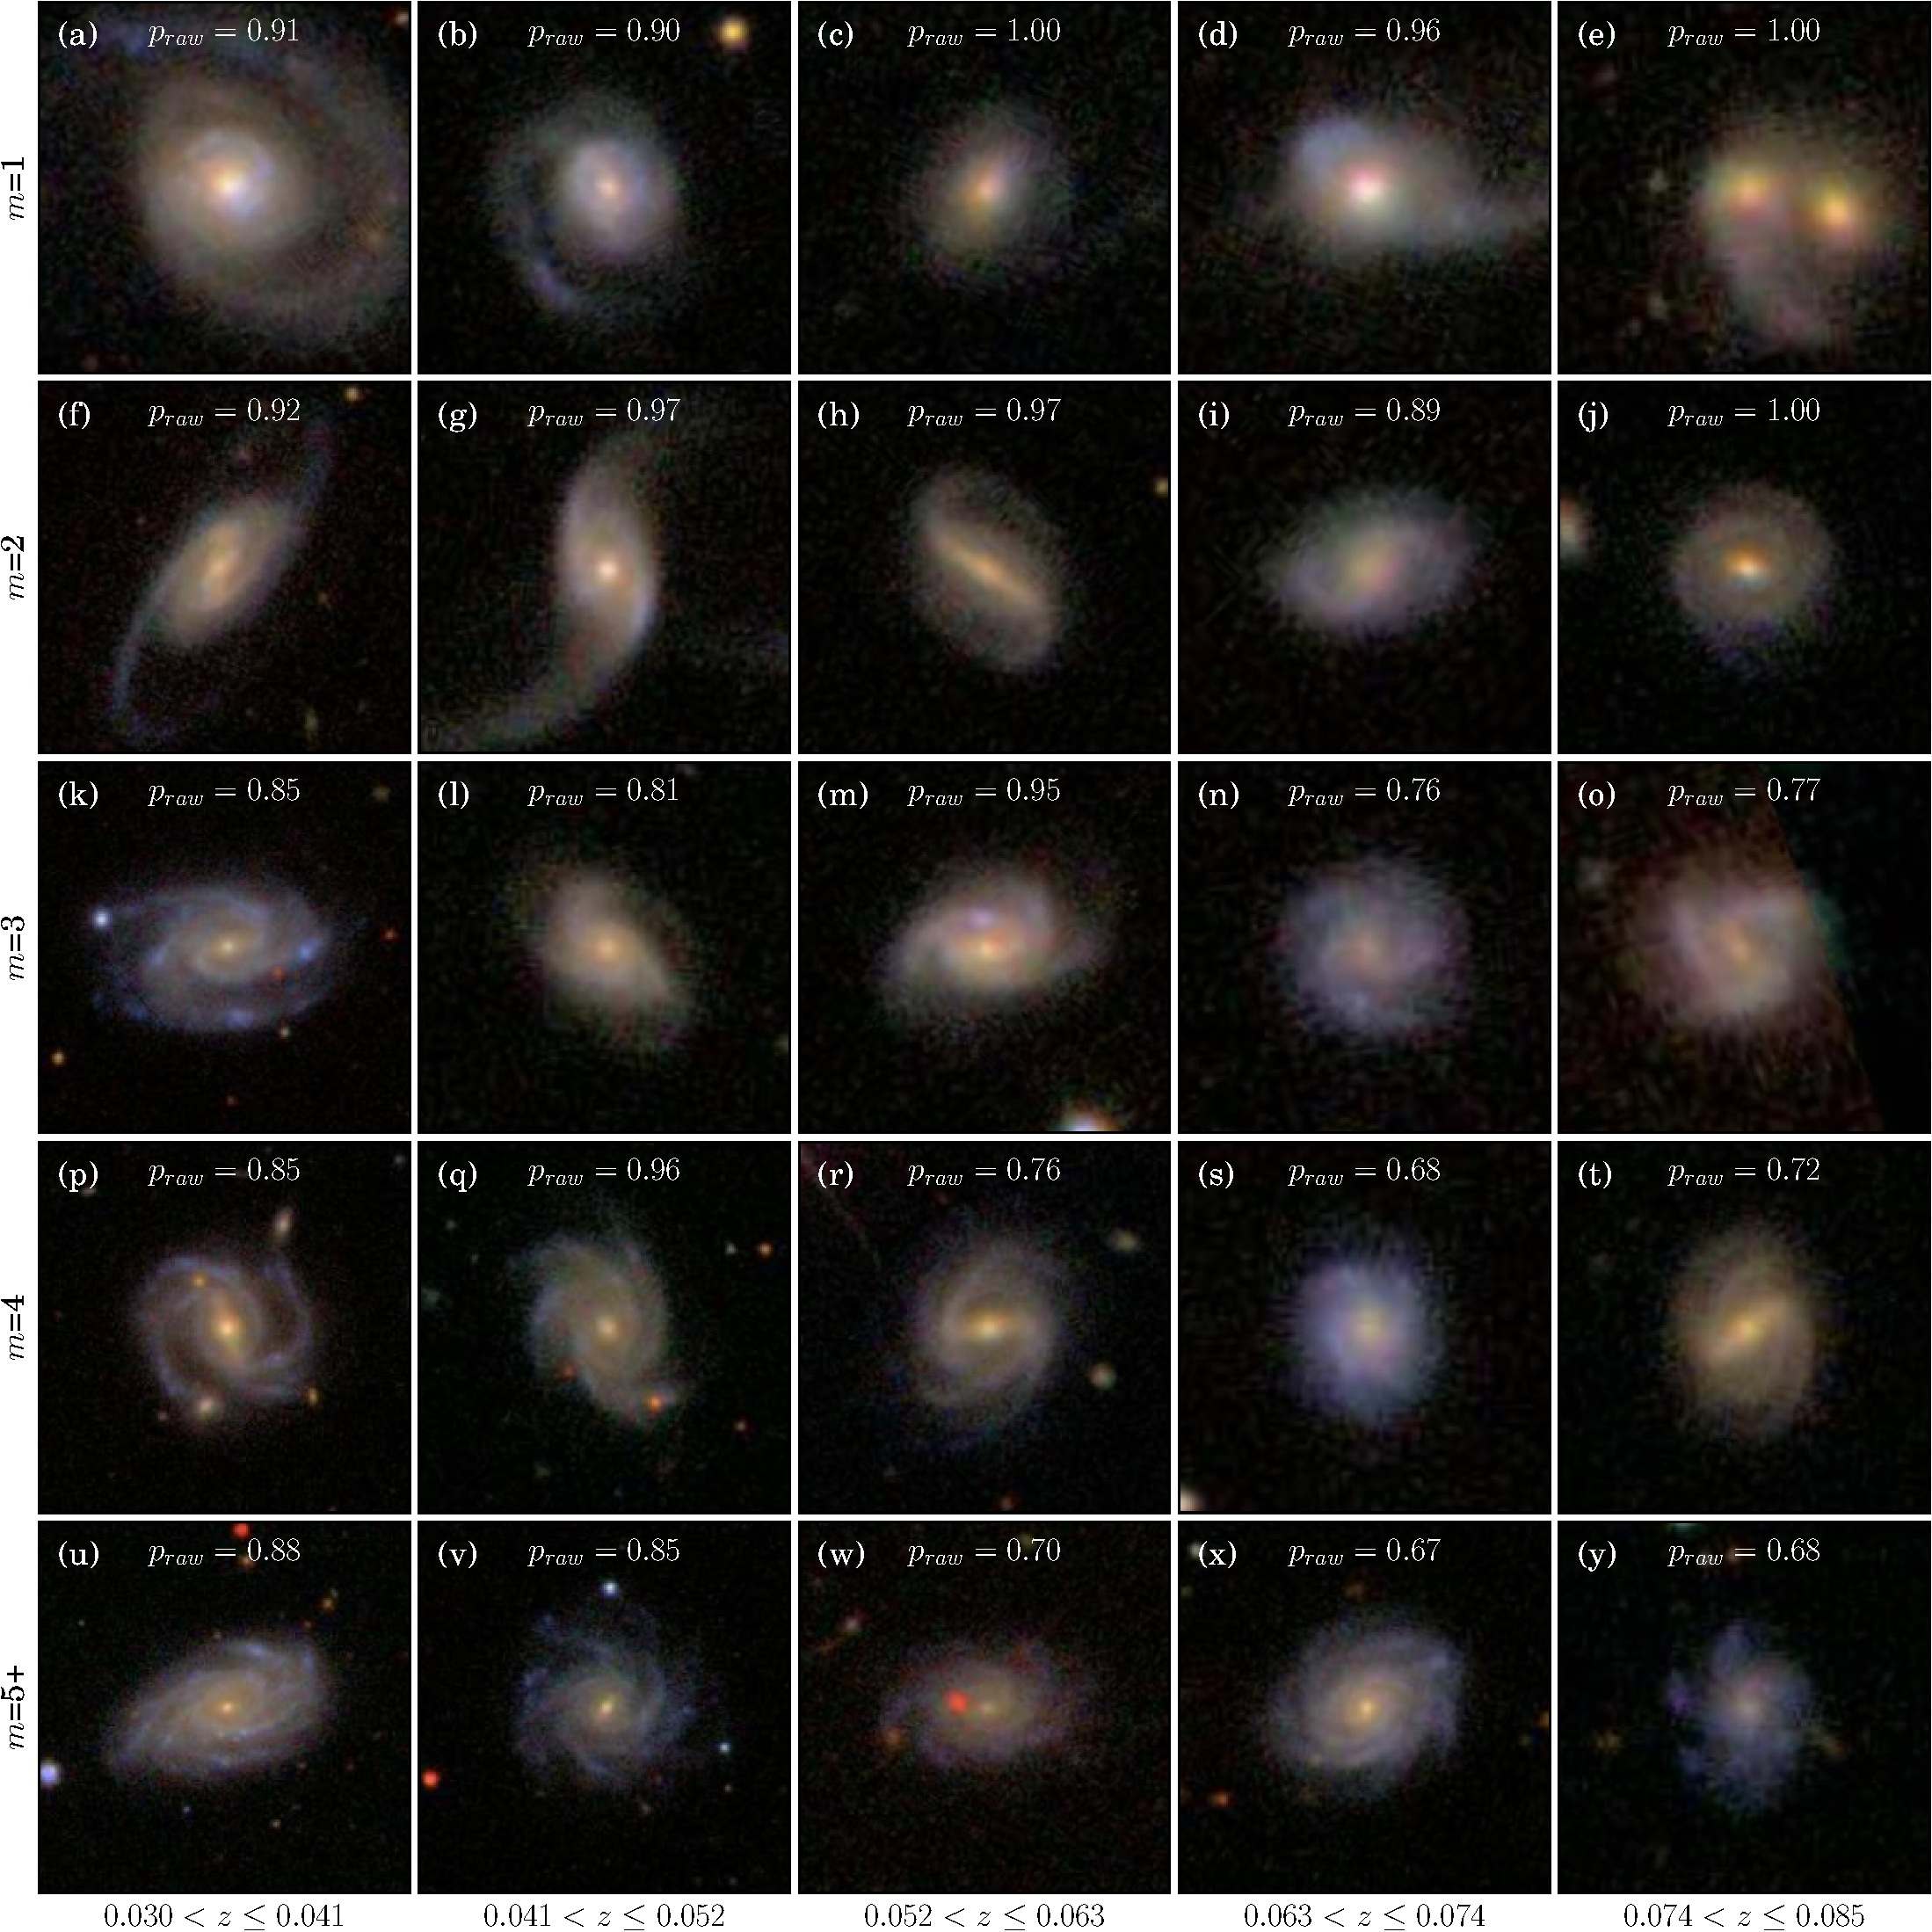
\includegraphics[width=0.975\textwidth]{Images/Results/image_page_p0810_m106110.pdf}

        \caption{Galaxies classified as 1,2,3,4 or more than 4 armed in different redshift ($z$) bins. Each of the galaxies is within a stellar mass range of $10.6 \leq \log(M/M_{\odot}) < 11.0$. Each of the galaxies has a modal $p$-value of $p_m > 0.8$.}

        \label{fig:image_panel_secure}

\end{figure*}

\begin{figure*}
		\centering

        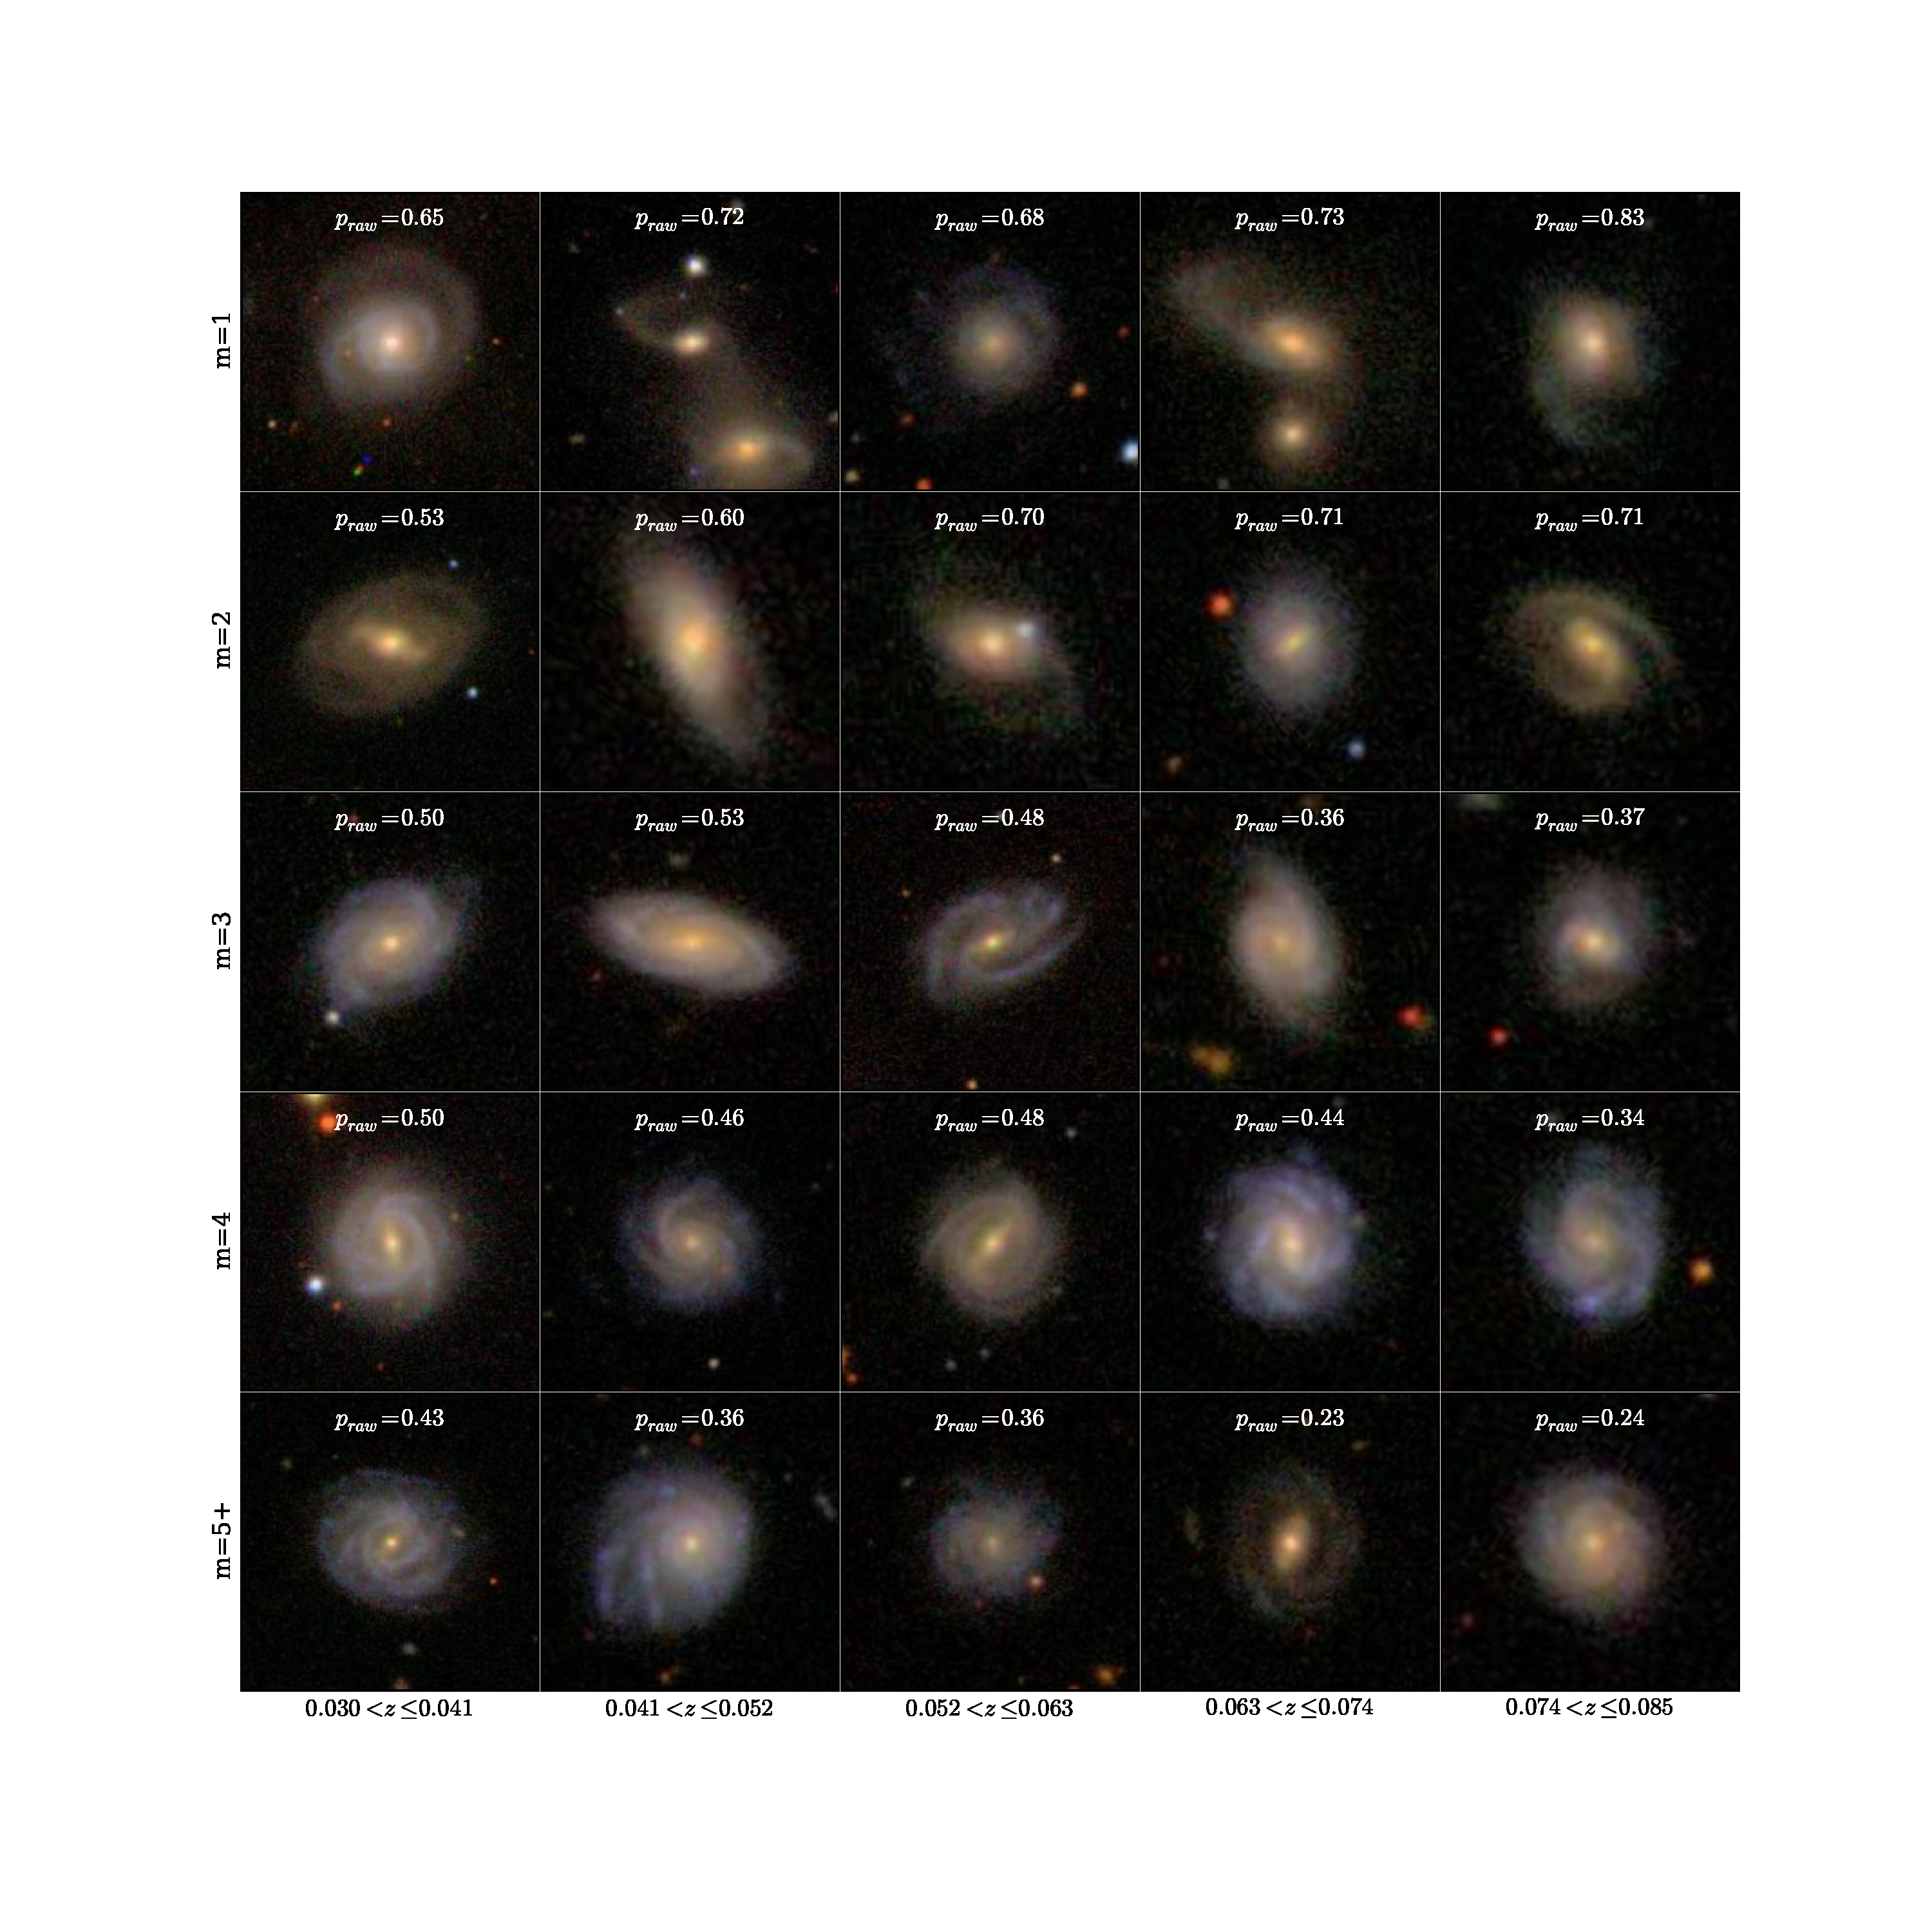
\includegraphics[width=0.975\textwidth]{Images/Results/image_page_p0506_m106110.pdf}

        \caption{Galaxies classified as 1,2,3,4 or more than 4 armed in different redshift ($z$) bins. Each of the galaxies is within a stellar mass range of $10.6 \leq \log(M/M_{\odot}) < 11.0$. The modal $p_m$ value (where $m$ is the spiral arm number) is within the range $0.5 \leq p_m < 0.6$.}

        \label{fig:image_panel}

\end{figure*}

In order for one to look in to how spiral properties vary in grand design and flocculent spirals, visual inspection of the number of arms in a spiral galaxy disk is required. Such classifications are provided by question T10 of the GZ2 question tree (see Fig.~\ref{fig:question_tree}). 

However, spiral arm multiplicity does not map exactly on to a specific Elmegreen-type for two reasons. Firstly, the arm number itself does not give any indication of the prominence of spiral arms, so cannot be used to distinguish between a galaxy with many well-defined arms and one with more flocculent spiral structure, which are usually defined differently \citep{EE_82,EE_87}. The second issue is that arm structure may not necessarily be consistent at all radii \citep{Grosbol_04} in a galaxy disk, and at all wavelengths \citep{Block_91,Block_94,Thornley_96}, meaning that assigning a single $m$-value of arm number may not give a complete picture of the overall spiral arm structure. The most `easy-to-map' categories may therefore be to compare our $m$=2 population with the galaxies classified as grand design, as grand design structure is usually associated with two well-defined arms across the entire disk \citep{EE_82}. In the \textit{luminosity-limited spiral sample}, $0.62$ \rh{errorbar?} of the galaxies show two-armed spiral structure. This result is consistent with optical visual classifications \citep{EE_82} and infra-red classifications \citep{Grosbol_04}, which suggest that $\sim 60\%$ of local spiral galaxies exhibit grand design spiral structure. 

In order to compare different spiral galaxies, a secure sample of spirals must first be defined. Galaxies with $p_{\textrm{features}} \times p_{\textrm{not edge-on}} \times p_{\textrm{spiral}} > 0.5$ are selected, corresponding to an overall $p>0.5$ sample. The samples made using these cuts from the \textit{luminosity-limited sample} and \textit{stellar mass-limited sample} are hereafter referred to as the \textit{stellar mass-limited spiral sample} and \textit{luminosity-limited spiral sample} respectively.

Each of the galaxies is then assigned a spiral arm number. Using the $p>0.5$ sample, defined above, a further cut is imposed where only galaxies with $N_{spiral} - N_{can't \, tell} \geq 5$ are selected. This means that the \textit{spiral sample} is only composed of galaxies where more than 5 individuals classified the spiral arm number, to reduce the effects of noise caused by low numbers of classifications. Each galaxy is then assigned a specific spiral arm number, $m$ of either 1,2,3,4 or 5+ arms, depending on which response has the highest debiased vote fraction (excluding the \textit{can't tell} response). Some examples of some securely classified spiral galaxies are shown in Fig.~\ref{fig:image_panel_secure}, where each galaxy has a dominant vote fraction of $p_m > 0.8$. The samples of galaxies assigned to each of the different $m$-values are hereafter referred to as the \textit{arm number samples}. 

The debiasing procedure applied to this question has shifted the vote fractions for the multiple-armed ($m$=3,4,5+) answers upwards overall, as can be seen in Fig.~\ref{fig:arm_number_trend}. This has the effect of making each of these samples more complete with redshift, by increasing their respective overall vote fractions. However, in the $m$=5+ arms case, the sample is still somewhat incomplete, as the overall fraction of galaxies that are assigned to this category decreases with redshift. This is because this categories vote distributions die off far more quickly with redshift than any of the other categories, as can be seen from the dashed line in the bottom panel of Fig.~\ref{fig:arm_number_trend}, making the  modelling of this redshift bias much more difficult. Despite this, the number and fraction of galaxies that make up the $m$=5+ category are still significantly improved compared to the sample sizes that would be defined using either the raw vote fractions or the W13 debiased vote fractions, as can be seen in from the $N$ and $f$ columns of table \ref{table:overall_property_table}. 

\begin{figure}
		\centering

        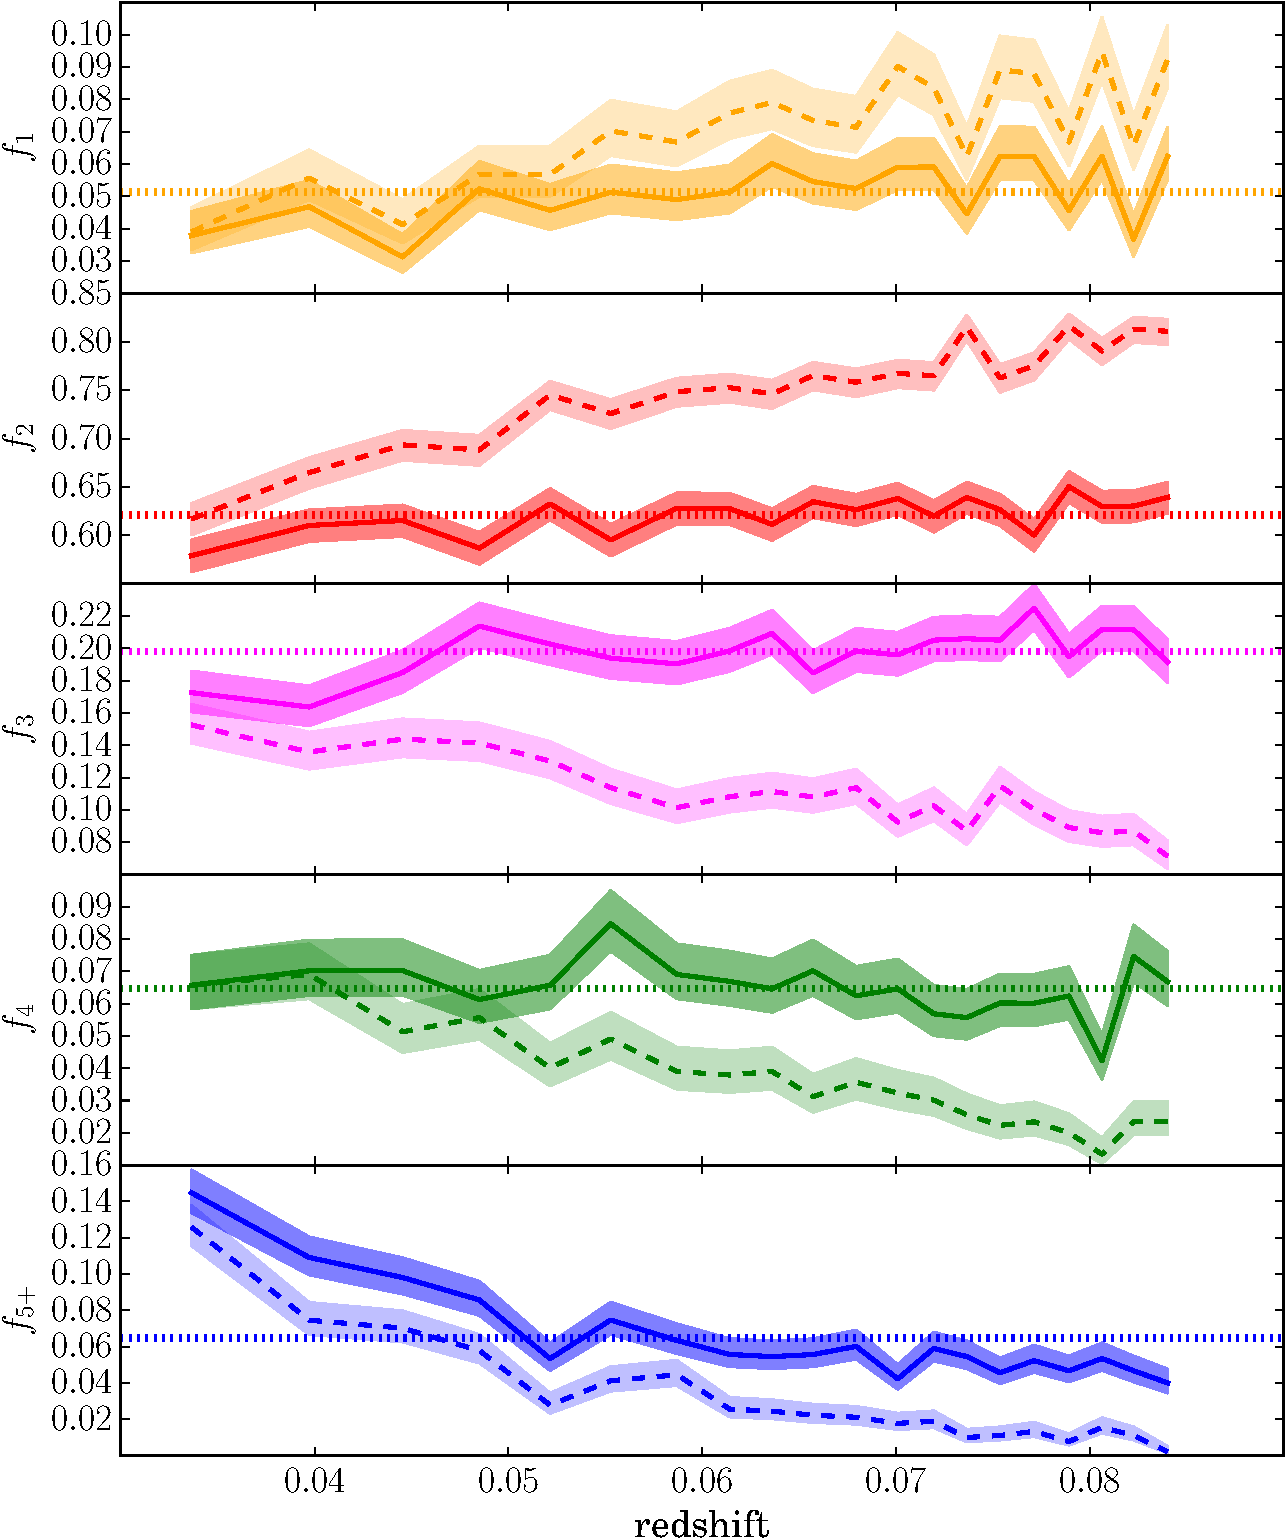
\includegraphics[width=0.45\textwidth]{Images/Results/sample_fractions.pdf}

        \caption{Fraction of galaxies in the \textit{luminosity-limited spiral sample} classified as having 1,2,3,4, or 5+ spiral arms as a function of redshift. The solid lines indicates the fractions from the debiased values, and the dashed line indicates the same fractions using the raw vote fractions. Errors are calculated using the method described in \citet{Cameron_11}. The horizontal dotted lines show the mean fractions using the debiased values averaged over all of the bins.}

        \label{fig:arm_number_trend}

\end{figure}

The main result of this debiasing is that galaxies with low vote fractions for the many-armed answers are shifted upwards so that they are included in the many-armed categories when they were not before. If this were not the case, then the fraction of $m$=2 galaxies would be contaminated by galaxies that actually have 3,4 or more than 4 spiral arms. This effect is evident in Fig.~\ref{fig:image_panel}, where a selection of spiral galaxies with $0.5 < p_m \leq 0.6$ are shown. It can be seen that the $m$=4 and $m$=5+ spiral samples at higher redshift are made up of spiral galaxies that initially had much lower overall vote fractions. As an example, if one were to select some `secure' galaxy samples with $p_m>0.5$, then the galaxy in the bottom right-hand corner of Fig.~\ref{fig:image_panel} would be unclassified, as its highest $p$-value would only be 
0.267 (for the $m$=4 response). Using our debiased values, it has a modal value of $p_m$=0.55 for the $m$=5+ armed response, so would be in the $m$=5+ sample. 

%------------------------------------------------------------------------------------
\subsection{Comparing overall galaxy populations}
\label{sec:comparison}

Having defined the samples of spiral galaxies in \S\ref{sec:defining_the_sample}, the demographics of the different galaxy populations separated by spiral arm number can be compared. Mean stellar mass ($M_*$), colour ($g-r$) and local densities ($\Sigma$) are tabulated in the final three columns of table~\ref{table:overall_property_table}.

\begin{table*}

\begin{tabular}{cccccccccc}
\hline
 $m$                    & $N_{raw}$   & $f_{raw}$   & $N_{W13}$   & $f_{W13}$   & $N_{debiased}$   & $f_{debiased}$   & $M_* (\log(M/M_{\odot}))$   & $g-r$            & $\Sigma \mathrm{(Mpc^{-2})}$  \\
\hline
 Luminosity-limited   & $12554$   & $1.00$    & $14297$   & $1.00$    & $17953$        & $1.00$         & $10.62\pm 0.25$                    & $0.58\pm 0.10$ & $10.62\pm 0.25$              \\
 1                    & $563$     & $0.04$    & $670$     & $0.05$    & $922$          & $0.05$         & $10.63\pm 0.27$                    & $0.58\pm 0.11$ & $10.63\pm 0.27$              \\
 2                    & $9044$    & $0.72$    & $10073$   & $0.70$    & $11150$        & $0.62$         & $10.63\pm 0.24$                    & $0.60\pm 0.10$ & $10.63\pm 0.24$              \\
 3                    & $1778$    & $0.14$    & $2158$    & $0.15$    & $3555$         & $0.20$         & $10.59\pm 0.26$                    & $0.53\pm 0.10$ & $10.59\pm 0.26$              \\
 4                    & $615$     & $0.05$    & $751$     & $0.05$    & $1162$         & $0.06$         & $10.60\pm 0.26$                    & $0.53\pm 0.09$ & $10.60\pm 0.26$              \\
 5+                   & $554$     & $0.04$    & $645$     & $0.05$    & $1164$         & $0.06$         & $10.65\pm 0.27$                    & $0.54\pm 0.09$ & $10.65\pm 0.27$              \\
 
\hline

 Stellar mass-limited & $6683$    & $1.00$    & $7226$    & $1.00$    & $9389$         & $1.00$         & $10.81\pm 0.16$                    & $0.63\pm 0.08$ & $10.81\pm 0.16$              \\
 1                    & $290$     & $0.04$    & $331$     & $0.05$    & $495$          & $0.05$         & $10.83\pm 0.16$                    & $0.65\pm 0.09$ & $10.83\pm 0.16$              \\
 2                    & $4852$    & $0.73$    & $5191$    & $0.72$    & $6039$         & $0.64$         & $10.81\pm 0.15$                    & $0.65\pm 0.07$ & $10.81\pm 0.15$              \\
 3                    & $886$     & $0.13$    & $991$     & $0.14$    & $1655$         & $0.18$         & $10.82\pm 0.16$                    & $0.59\pm 0.07$ & $10.82\pm 0.16$              \\
 4                    & $335$     & $0.05$    & $366$     & $0.05$    & $564$          & $0.06$         & $10.82\pm 0.16$                    & $0.58\pm 0.07$ & $10.82\pm 0.16$              \\
 5+                   & $320$     & $0.05$    & $347$     & $0.05$    & $636$          & $0.07$         & $10.85\pm 0.18$                    & $0.58\pm 0.07$ & $10.85\pm 0.18$              \\
\hline
\end{tabular}



\caption{Overall properties of galaxy populations with different numbers of spiral arms. The number of galaxies with 1,2,3,4 and more than 4 arms are shown for both the \textit{luminosity-limited} and \textit{stellar mass-limited spiral samples}. Mean stellar masses, colours and star-formation rates are shown for each of the populations, with $1\sigma$ standard deviations.}

\label{table:overall_property_table}

\end{table*}

%------------------------------------------------------------------------------------
\subsubsection{Stellar mass}
\label{sec:mass}

\begin{figure*}
		\centering

        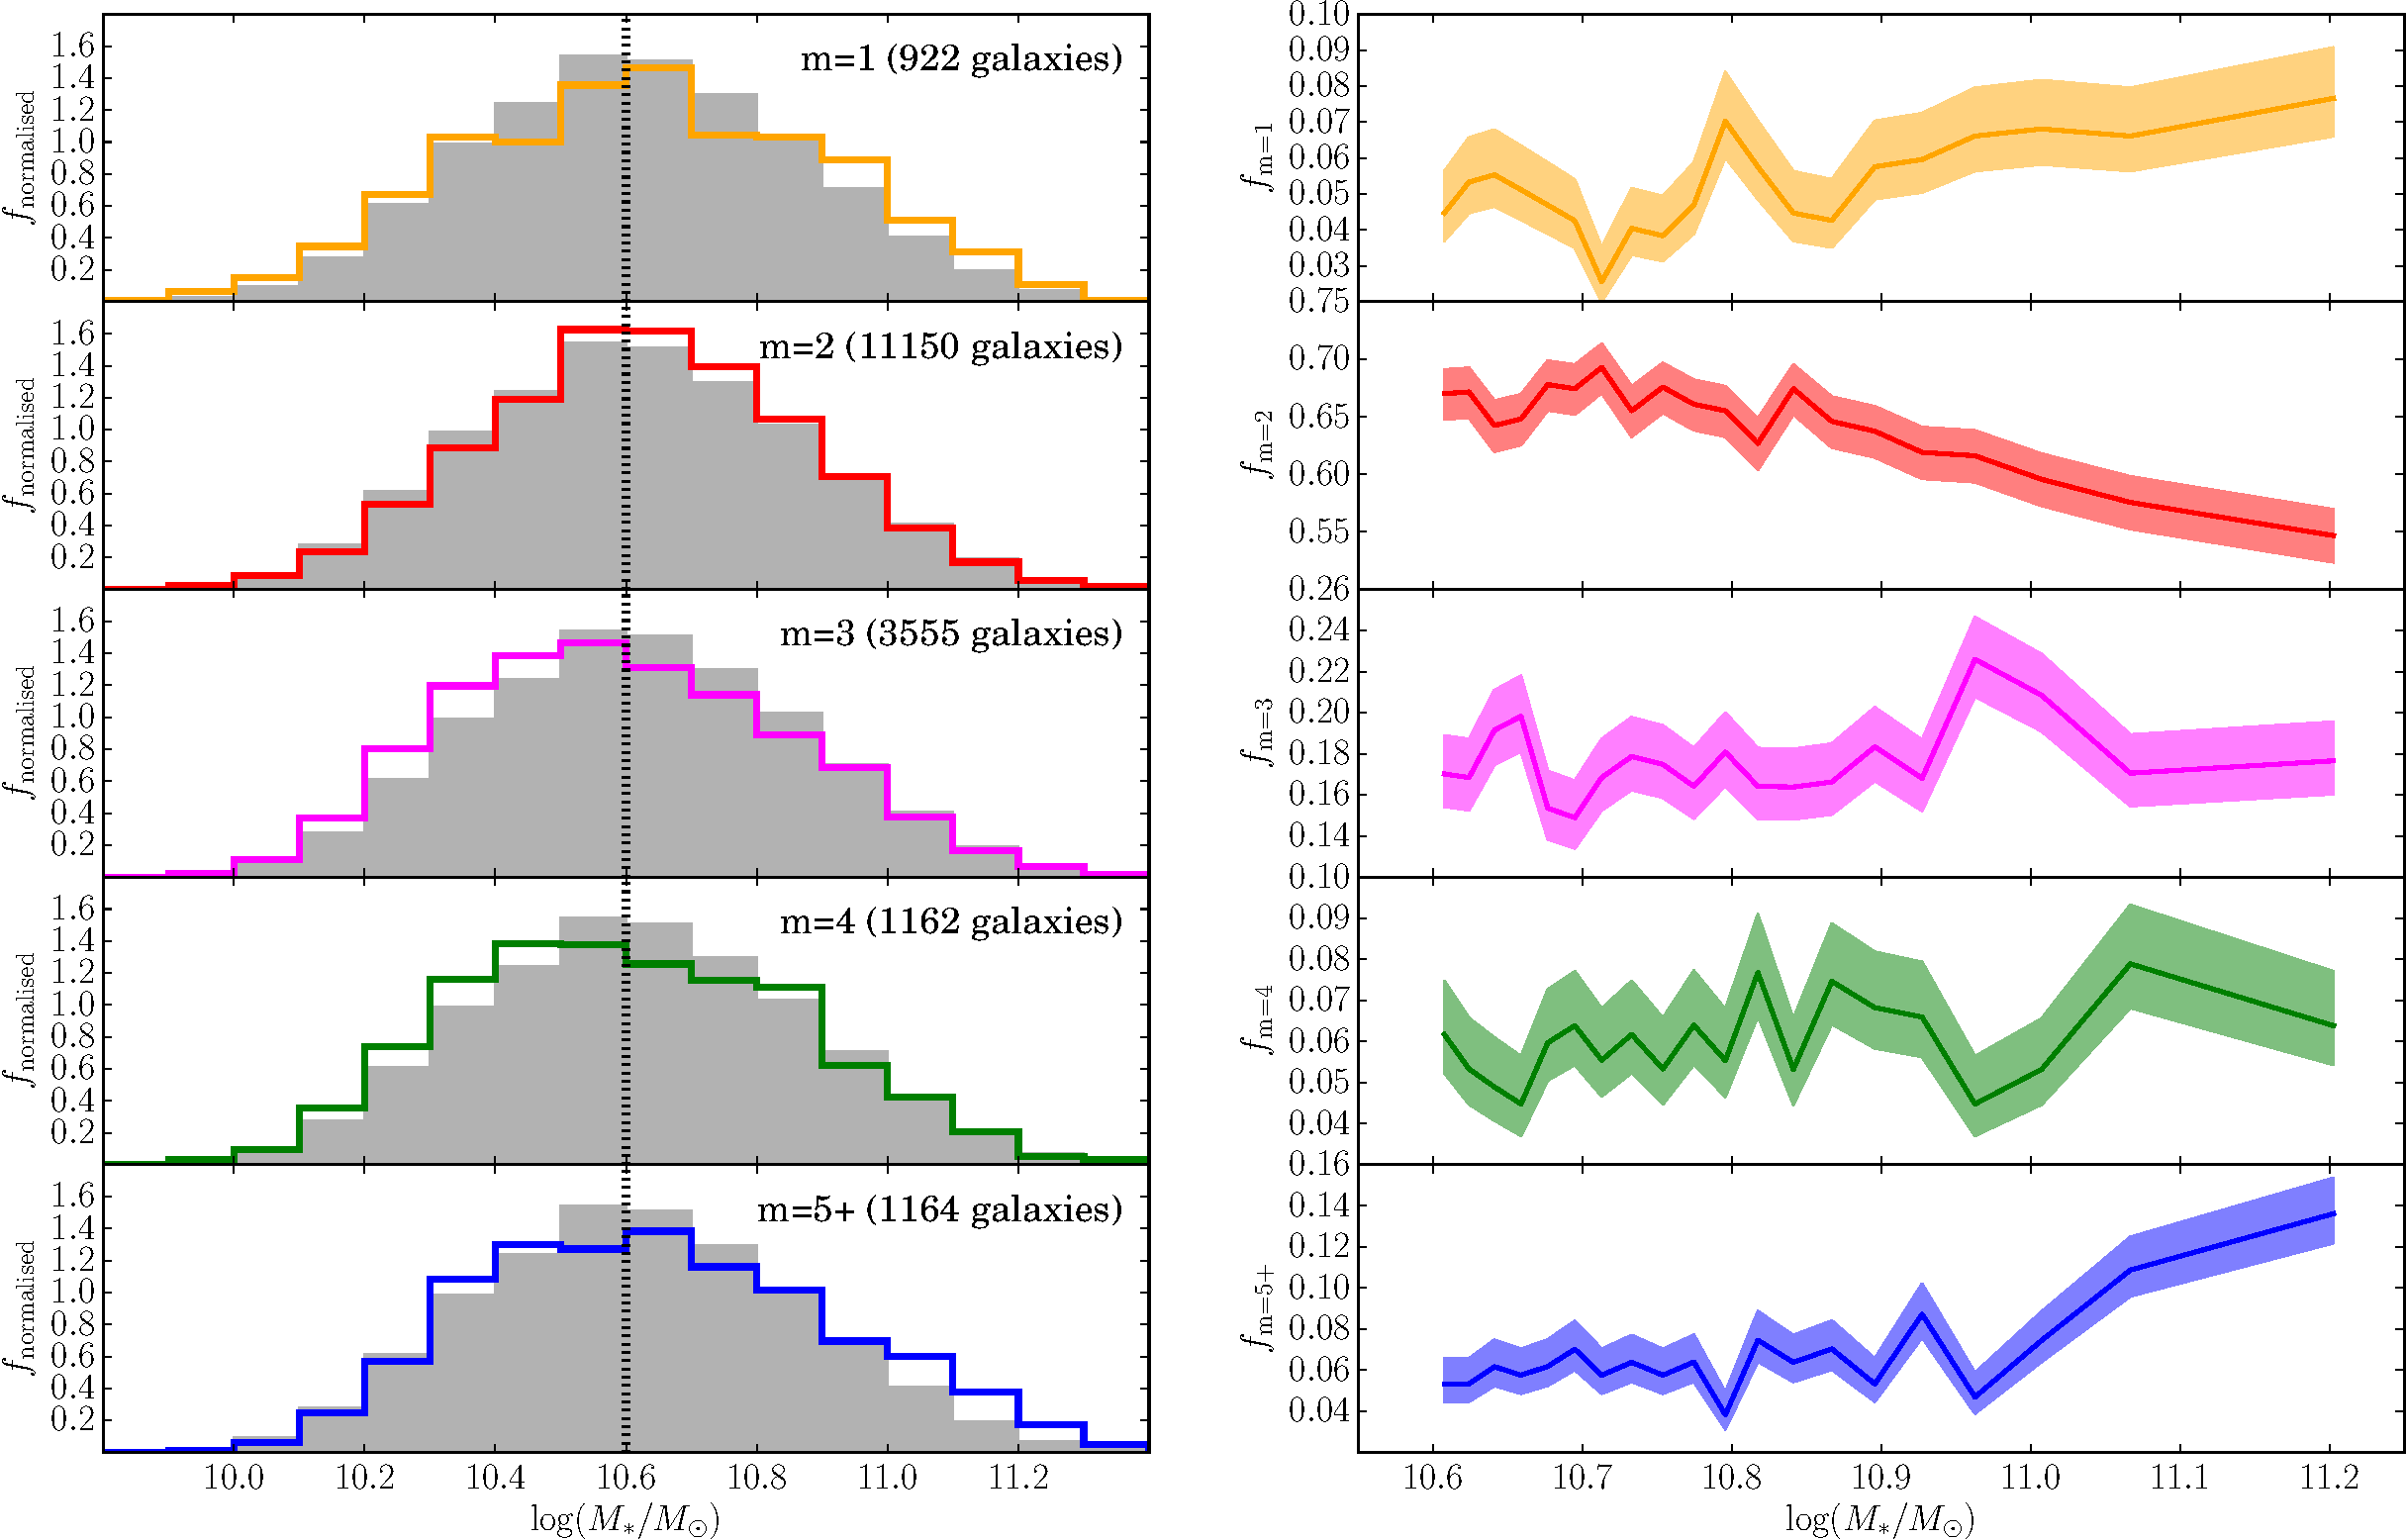
\includegraphics[width=0.975\textwidth]{Images/Results/mass_plots.pdf}

        \caption{Left: distributions of stellar mass for the \textit{luminosity-limited spiral sample}. The solid lines indicate the distributions for each of the \textit{arm number samples} for each of arm numbers. The grey filled histograms show the equivalent distribution for all of the spiral galaxies for reference. The black dotted line indicates the stellar mass values above which the sample is complete in stellar mass. Right: fraction of the \textit{stellar mass-limited spiral sample} classified as having each spiral arm number, in 20 bins of stellar mass. The shaded regions indicate the 1$\sigma$ error calculated using the method described in \citet{Cameron_11}.}

        \label{fig:mass_plots}

\end{figure*}

Galaxy stellar mass is known to correlate with galaxy morphology \citep{Bamford_09,Kelvin_14}, and spiral galaxy Hubble-type \citep{Munoz-Mateos_15}. It has also been shown that stellar mass correlates with the strength of the $m$=2 mode in spiral galaxies, with two-armed structure more common in galaxies with greater physical size \citep{EE_87} and stellar mass \citep{Kendall_15}. The distributions of stellar mass for each of the \textit{arm number samples} are shown in Fig.~\ref{fig:mass_plots}a. The overall distributions for each of the galaxy samples show that there is no absolute dependence of spiral arm number with respect to host galaxy stellar mass; each of the samples contains galaxies across the entire range of stellar mass from $10.0 \lesssim \log(M_*/M_{\odot}) \lesssim 11.5$. 

The distributions of Fig.~\ref{fig:mass_plots}a show the overall distributions from the \textit{luminosity-limited spiral sample}, so are therefore incomplete for low stellar mass galaxies (see \S\ref{sec:sample}). To look for trends in terms of stellar mass, the overall fraction of the \textit{stellar mass-limited spiral sample} is shown in Fig.~\ref{fig:mass_plots}b. In this case, it can be seen that there does appear to be a relation of spiral arm number as a function of host galaxy stellar mass. A significant increase in the fraction of galaxies with 5+ spiral arms is observed from the overall mean value of $0.068 \pm 0.003$ to $0.14 \pm 0.02$ for the highest stellar mass bin of $\log(M/M_{\odot}) = 11.2 \pm 0.1$. Conversely, the fraction of galaxies with two spiral arms decreases from $0.643 \pm 0.005$ for the total population to $0.55 \pm 0.02$ in the highest stellar mass bin. 

The first reason for why higher mass spirals may exhibit more spiral arms is that this could purely be an effect from the visual classifications. It has already been  identified that the many-armed spiral features are the most difficult to detect, so  may be more easily identifiable in the largest, brightest spiral galaxies. Another interesting scenario may be that the population of galaxies with the highest stellar mass are a population of unquenched spiral galaxies as in \citealt{Ogle_16}. Such galaxies may not have undergone a `quenching' mechanism, which may be responsible for the transformation of many-armed spiral structure to two-armed spiral structure. If such galaxies had massive disks (and therefore low bulge-to-total masses) would also mean that higher spiral arm modes are favoured \citep{Donghia_15}.
%------------------------------------------------------------------------------------
\subsubsection{Local environment}
\label{sec:environment}

\begin{figure*}
		\centering

        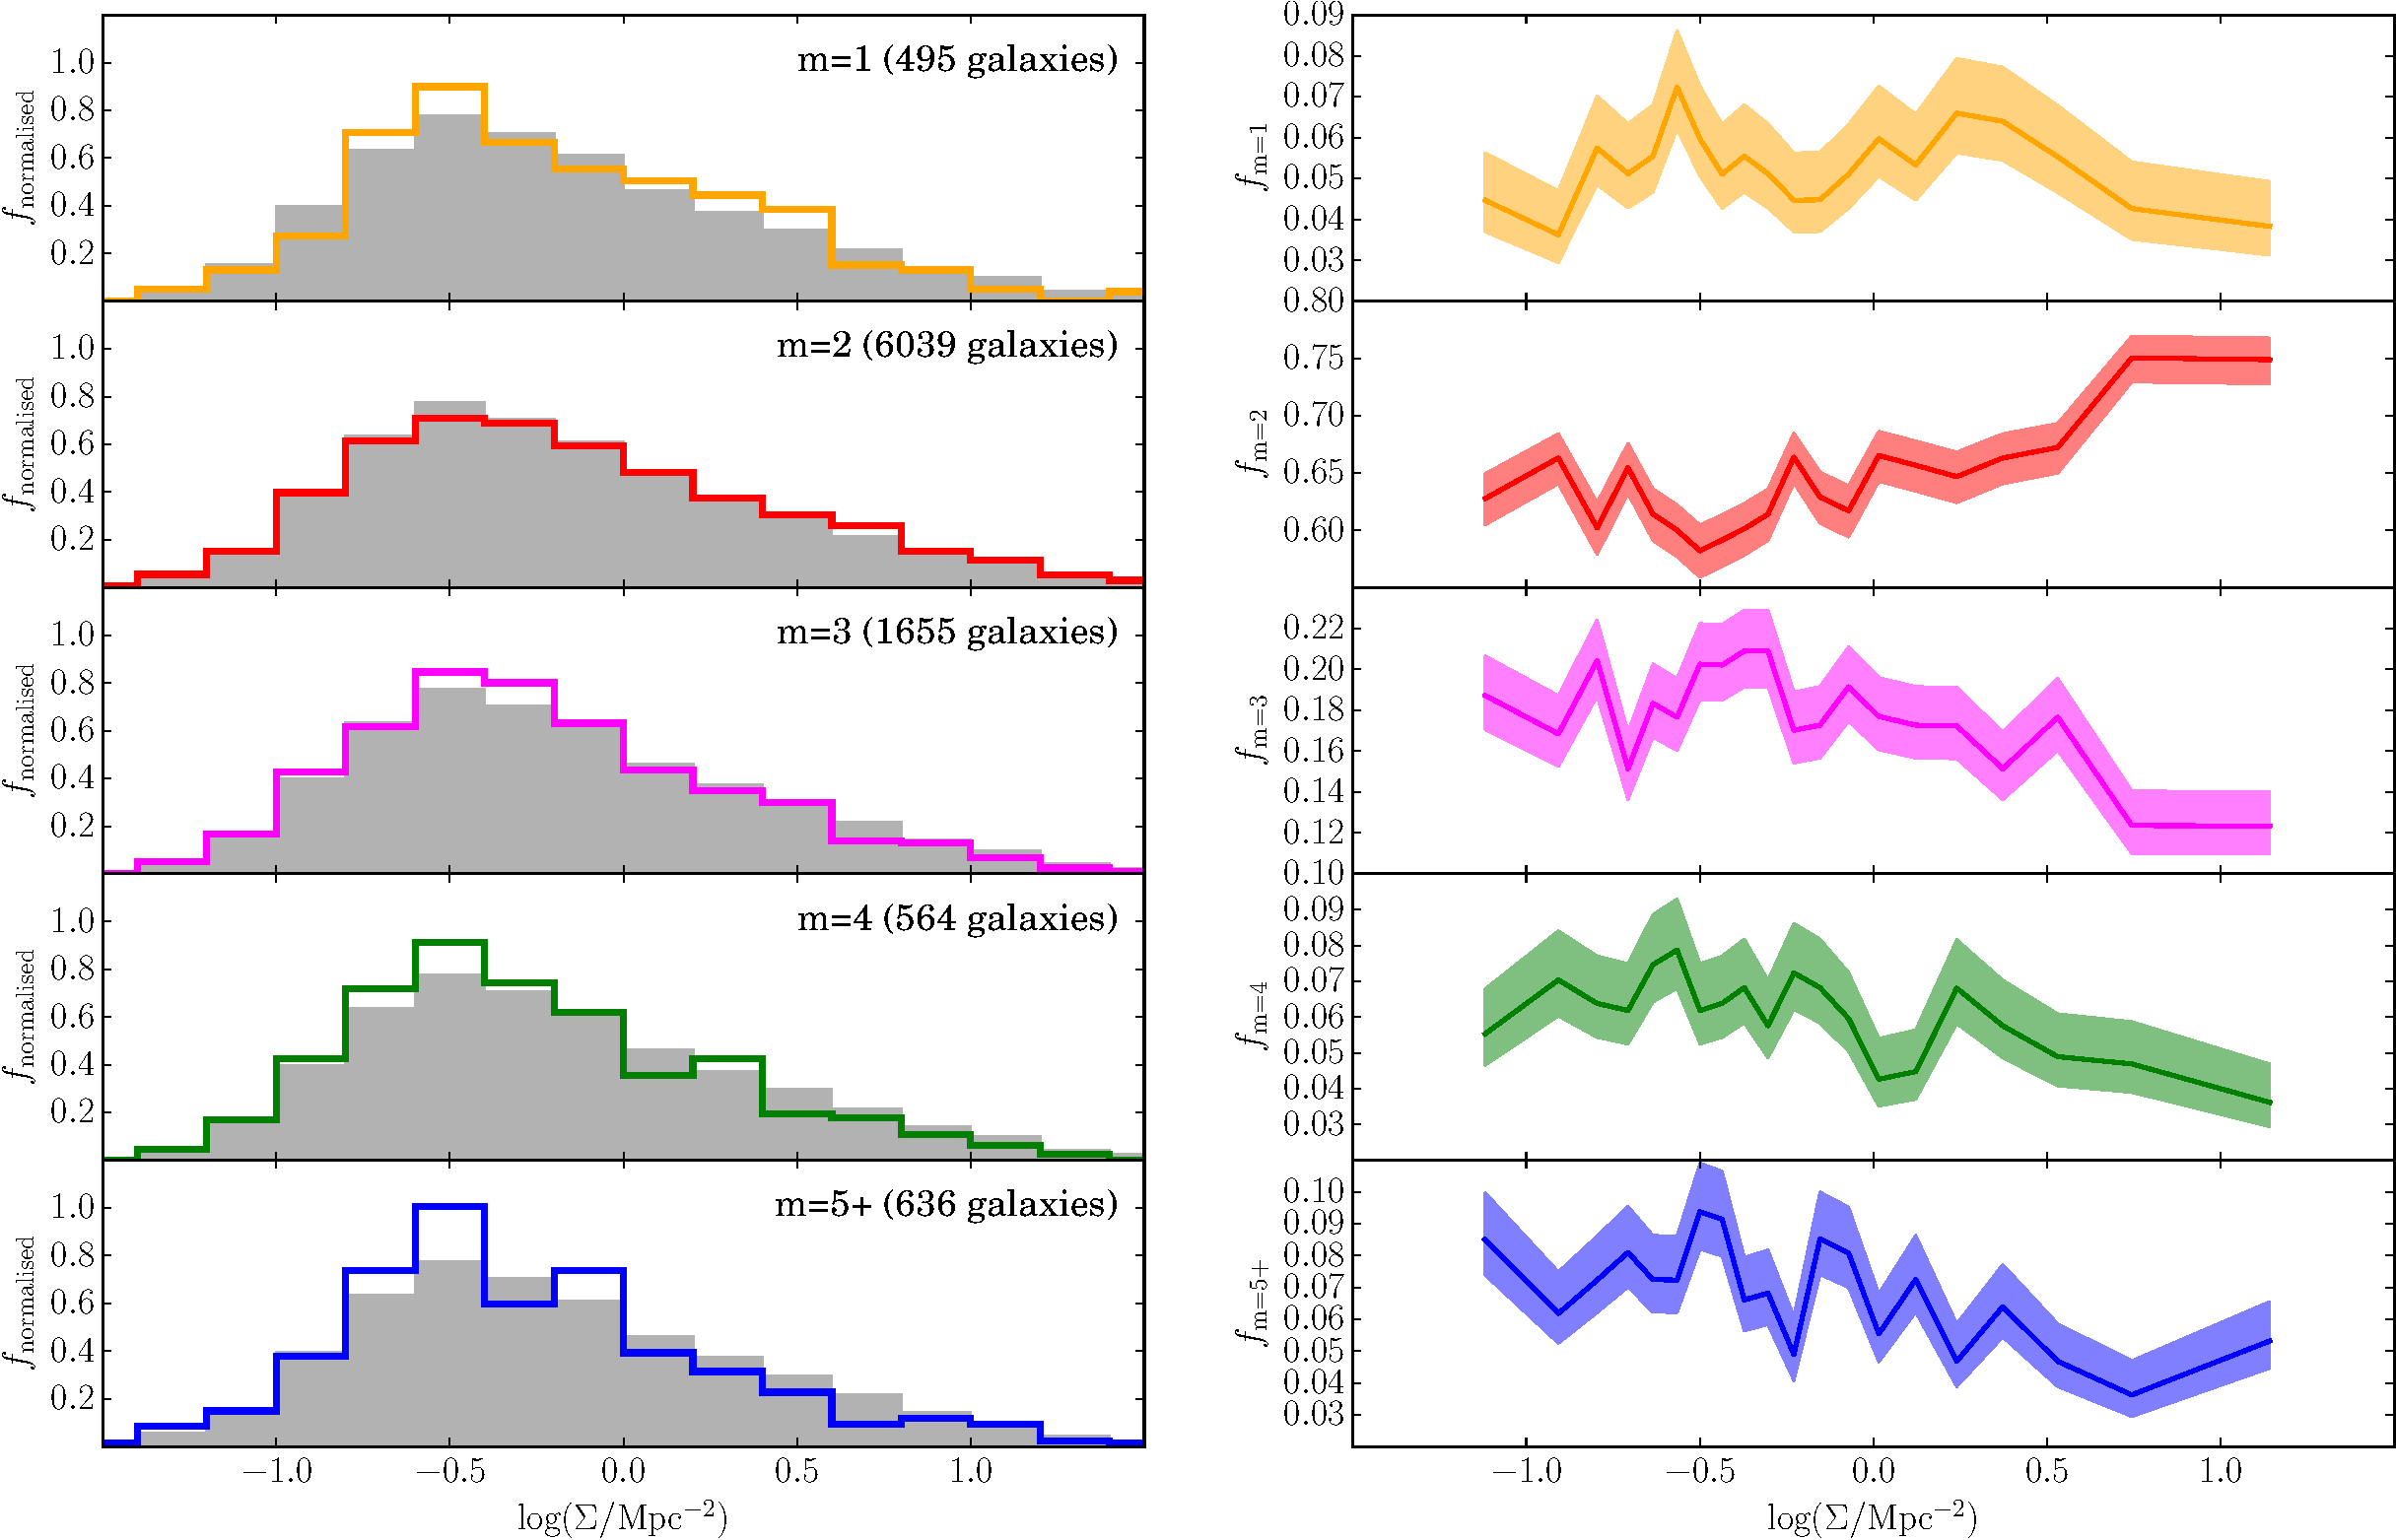
\includegraphics[width=0.975\textwidth]{Images/Results/density_plots.pdf}

        \caption{Left: distributions of local density ($\Sigma$) for the \textit{stellar mass-limited spiral sample}. The solid lines indicate the distributions for each of the \textit{arm number samples} for each of arm numbers. The grey filled histograms show the equivalent distribution for all of the spiral galaxies for reference. Right: fraction of the \textit{stellar mass-limited spiral sample} classified as having each spiral arm number, in 20 bins of $\Sigma$. The shaded regions indicate the 1$\sigma$ error calculated using the method described in \citet{Cameron_11}.}

        \label{fig:density_plots}

\end{figure*}

It is already well established that there is a clear dependence of the type of spiral structure that galaxies exhibit with respect to their local environment. Observational evidence from comparison of visually classified galaxies has found that grand design galaxies are more prominent in high density group environments \citep{EE_82,EE_87,Ann_14} and in binary systems where a close companion galaxy is present \citep{EE_82,Ann_14}. These results suggest that a mechanism is responsible for the transformation of spiral structure as galaxies enter the highest density environments, with a plausible explanation being that two-armed spiral structure is the result of a recent interaction between spiral galaxies. N-body modelling of galaxies has shown that two-armed spiral structure can occur as a result of galaxy-galaxy interactions, resulting in a disk displaying the two-armed grand design spiral structure that we see in the local Universe \citep{Sundelius_87,Dobbs_10}. However, the timescales of the persistence of such structures are thought to be relatively short-lived \citep{Oh_08,Dobbs_10}, meaning that an enhancement in the fraction of grand design galaxies is only observed in the highest density environments where interactions can happen on a frequent enough basis to sustain such structures \citep{EE_86}.

To compare spiral arm structure as a function of environment, a mean of $\Sigma_4$ and $\Sigma5$ is used as an estimate of local density, as in \citealt{Baldry_06}. This measure of local density will be hereafter denoted as $\Sigma$. This measure of local environment has been used to recover trends of environment with respect to galaxy properties before \citep{Baldry_06,Bamford_09}. \rh{Why is this a good measure of environment???}.

The overall distributions of galaxy local densities for each of the \textit{arm number samples} are shown in Fig.~\ref{fig:density_plots}a. Here, the \textit{stellar mass-limited spiral sample} is used to define the total population, as $M_*$ and density are closely related \citep{Baldry_06}, so any biases in terms of the stellar mass distributions may have an effect on the completeness of the galaxy sample in terms of environment. The overall distributions show a qualitatively similar result to the results of stellar mass- there is no absolute dependence of spiral arm number with local density. 

The fraction of spiral galaxies which exhibit each of the spiral arm numbers with respect to stellar mass are shown in Fig.~\ref{fig:density_plots}b. A clear trend of spiral arm number with respect to local density is observed, with the number of two-armed spiral galaxies increasing for the highest values of local density from $0.643 \pm 0.05$ for the overall population to $0.75 \pm 0.02$ for the highest density bin of $\log \Sigma = 1.1 \pm 0.2$. These results are in close agreement with those from \citealt{EE_82} and \citealt{Ann_14}, in which the fraction of galaxies displaying grand design spiral structure increases in the highest density environments. As the increase seems to be most distinct in the very highest density environments, this could be indicative that two-armed spiral structure is a  short-lived phase induced by galaxy-galaxy interactions, as described in \citealt{EE_86}. A more complete analysis of spiral structure with local environment, taking into account both interaction probabilities and overall density, would need to be considered to test this hypothesis.


%------------------------------------------------------------------------------------
\subsubsection{Galaxy colours}
\label{sec:colours}

\begin{figure*}
		\centering

        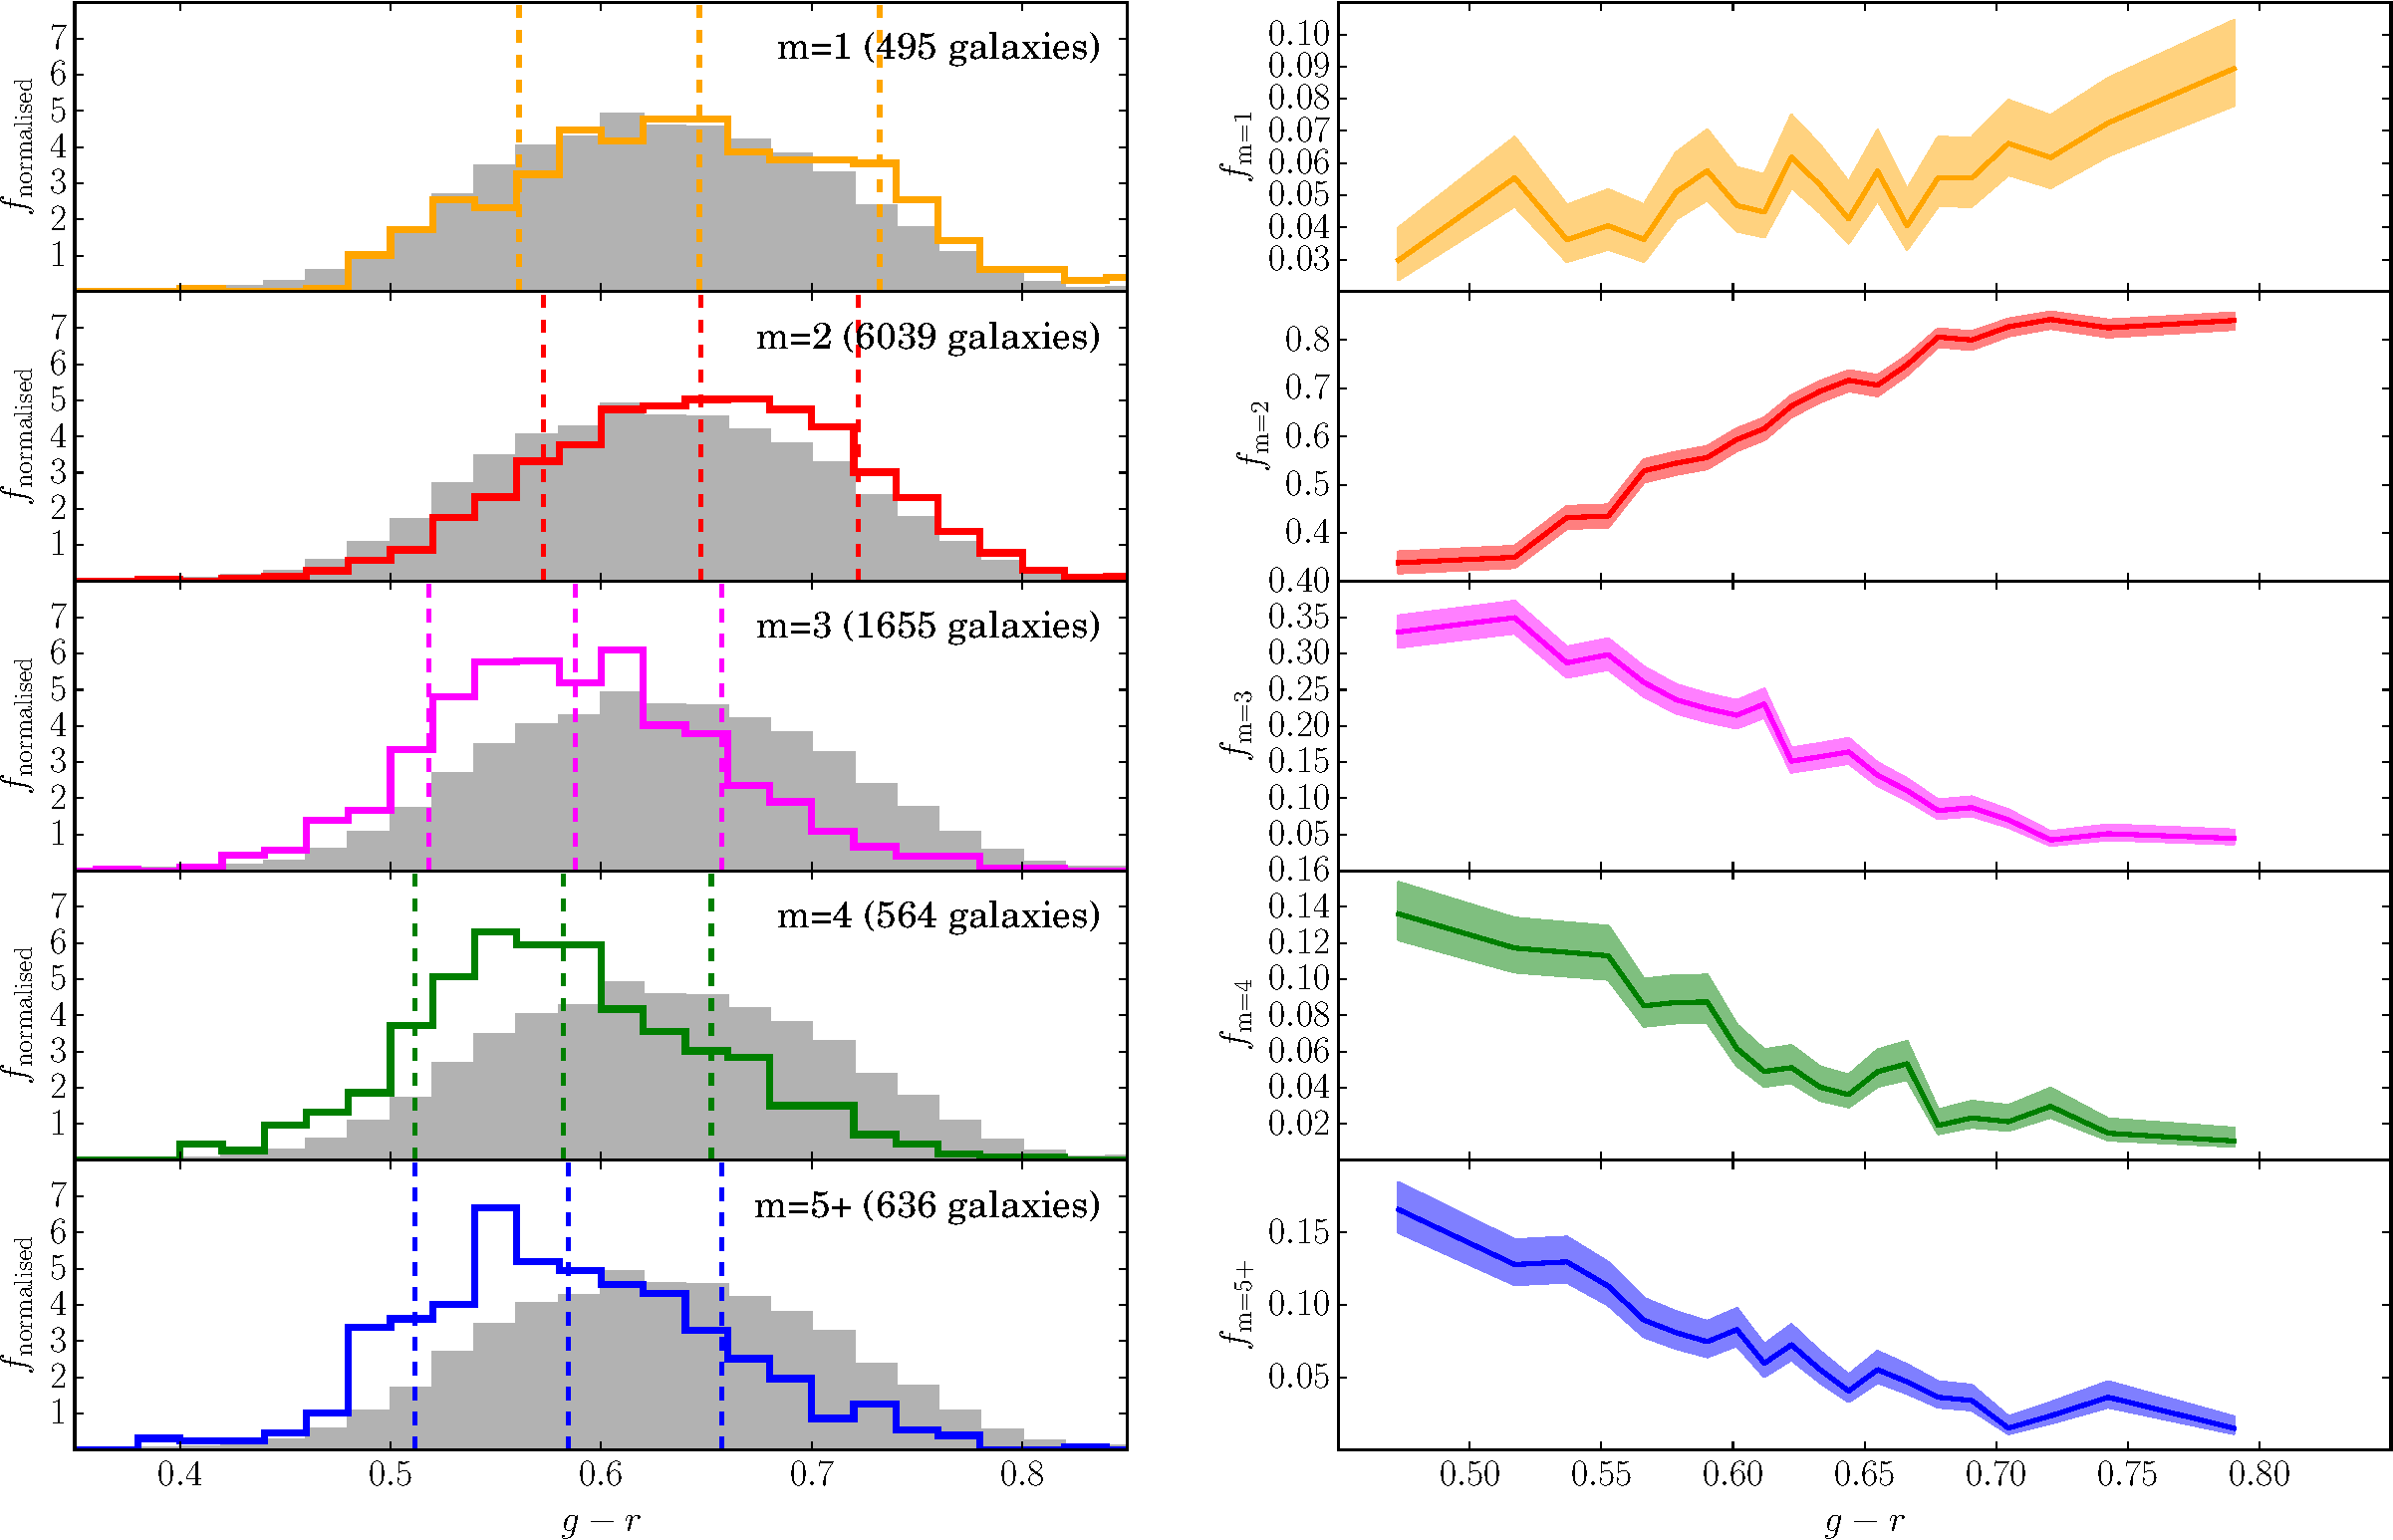
\includegraphics[width=0.975\textwidth]{Images/Results/colour_plots.pdf}

        \caption{Left: distributions of $g-r$ colour for the \textit{stellar mass-limited spiral sample}. The solid lines indicate the distributions for each of the \textit{arm number samples} for each of arm numbers. The grey filled histograms show the equivalent distribution for all of the spiral galaxies for reference. Right: fraction of the \textit{stellar mass-limited spiral sample} classified as having each spiral arm number, in 20 bins of $g-r$. The shaded regions indicate the 1$\sigma$ error calculated using the method described in \citet{Cameron_11}.}

        \label{fig:colour_plots}

\end{figure*}

Comparing the properties of spiral galaxies with respect to colour has been used in the past to test overall star-formation properties. By observing the NUV-optical colours of grand design spiral galaxies, it has been found that there is no significant enhancement in recent star-formation activity in two-armed spiral galaxies \citep{Romanishin_85,EE_86}. These results have since been verified, as there is also no enhancement of the star-formation in the individual arms of grand design spirals \citep{Foyle_11,Choi_15}. 

Galaxy colour is already known to relate to stellar mass \citep{Baldry_06}, environment \citep{Baldry_04} and overall galaxy morphology \citep{Bamford_09}. As trends with both stellar mass (\S~\ref{sec:mass}) and local environment (\S~\ref{sec:environment}) have already been found, the colour distributions are now compared to look for any further trends with star formation in Fig.~\ref{fig:colour_plots}a. The colours that are plotted here are the $g-r$ colours, covering a broad range of the optical spectrum. Unlike the distributions of local density and stellar mass, a strong trend is found with colour and arm multiplicity. The two-armed spiral galaxies show the reddest overall colours of $0.65 \pm 0.07$ in the stellar mass limited sample. The $m=3$,$m=4$ and $m=5+$ armed samples have corresponding colours of $0.59 \pm 0.07$,$0.58 \pm 0.07$ and $0.58 \pm 0.07$ respectively corresponding to a shift of approximately $1\sigma$ in comparison.

To further compare the overall galaxy colours, the fraction of the \textit{stellar mass-limited spiral sample} with each of the spiral arm numbers with respect to $g-r$ is shown in Fig.~\ref{fig:colour_plots}b. Here, a clear trend is observed with the fraction of galaxies displaying two spiral arms with respect to colour. In the bluest bin of $g-r=0.47 \pm 0.03$, only $0.34 \pm 0.02$ of galaxies have two spiral arms; in the reddest bin of $g-r=0.79 \pm 0.05$, $0.84 \pm 0.02$ have two spiral arms.

Using a single colour only gives an indication as to how the star-formation properties of galaxies differ, as redder optical colours could be the result of either enhanced star-formation \rh{cite} or an older overall stellar population \rh{cite}. To try to gain more of a physical understanding of how the stellar populations of spiral galaxies with different numbers of spiral arms differ, the $u-r$ and $r-z$ bands are compared for each of the different arm numbers, and the results are plotted in Fig.~\ref{fig:colour-colour}. From this plot, it can be seen that the most significant colour differences are observed in the $r-z$ band, which traces the older stellar population, rather than than the $u-r$ band, which traces the younger stellar population. The most significant differences are observed between the $m=2$ and $m=5+$ samples, where there is a significant offset in $r-z$ for a given $u-r$. In order to gain more physical insight, the two distributions are plotted against each other directly in Fig.~\ref{fig:cc_w_sfh}. The plot also includes BC03 $t$ and $\tau$ star-formation history (SFH) models for reference \rh{cite}. The plot indicates that both of the stellar populations can be well-fitted by SFH models of galaxies undergoing quenching, but that the process started earlier in the $m$=2 population than in the $m$=5+ population, meaning that the $m$=2 population is more `quenched'. The optical thickness of the galaxies could also play a significant role, as dust extinction could also account for much of the differences in the galaxy colours. Differences in optical thickness with respect to Hubble-type have been found before \citep{Ma_02}, so the possibility that there may be a correlation with arm multiplicity must also be considered.

\begin{figure*}
		\centering

        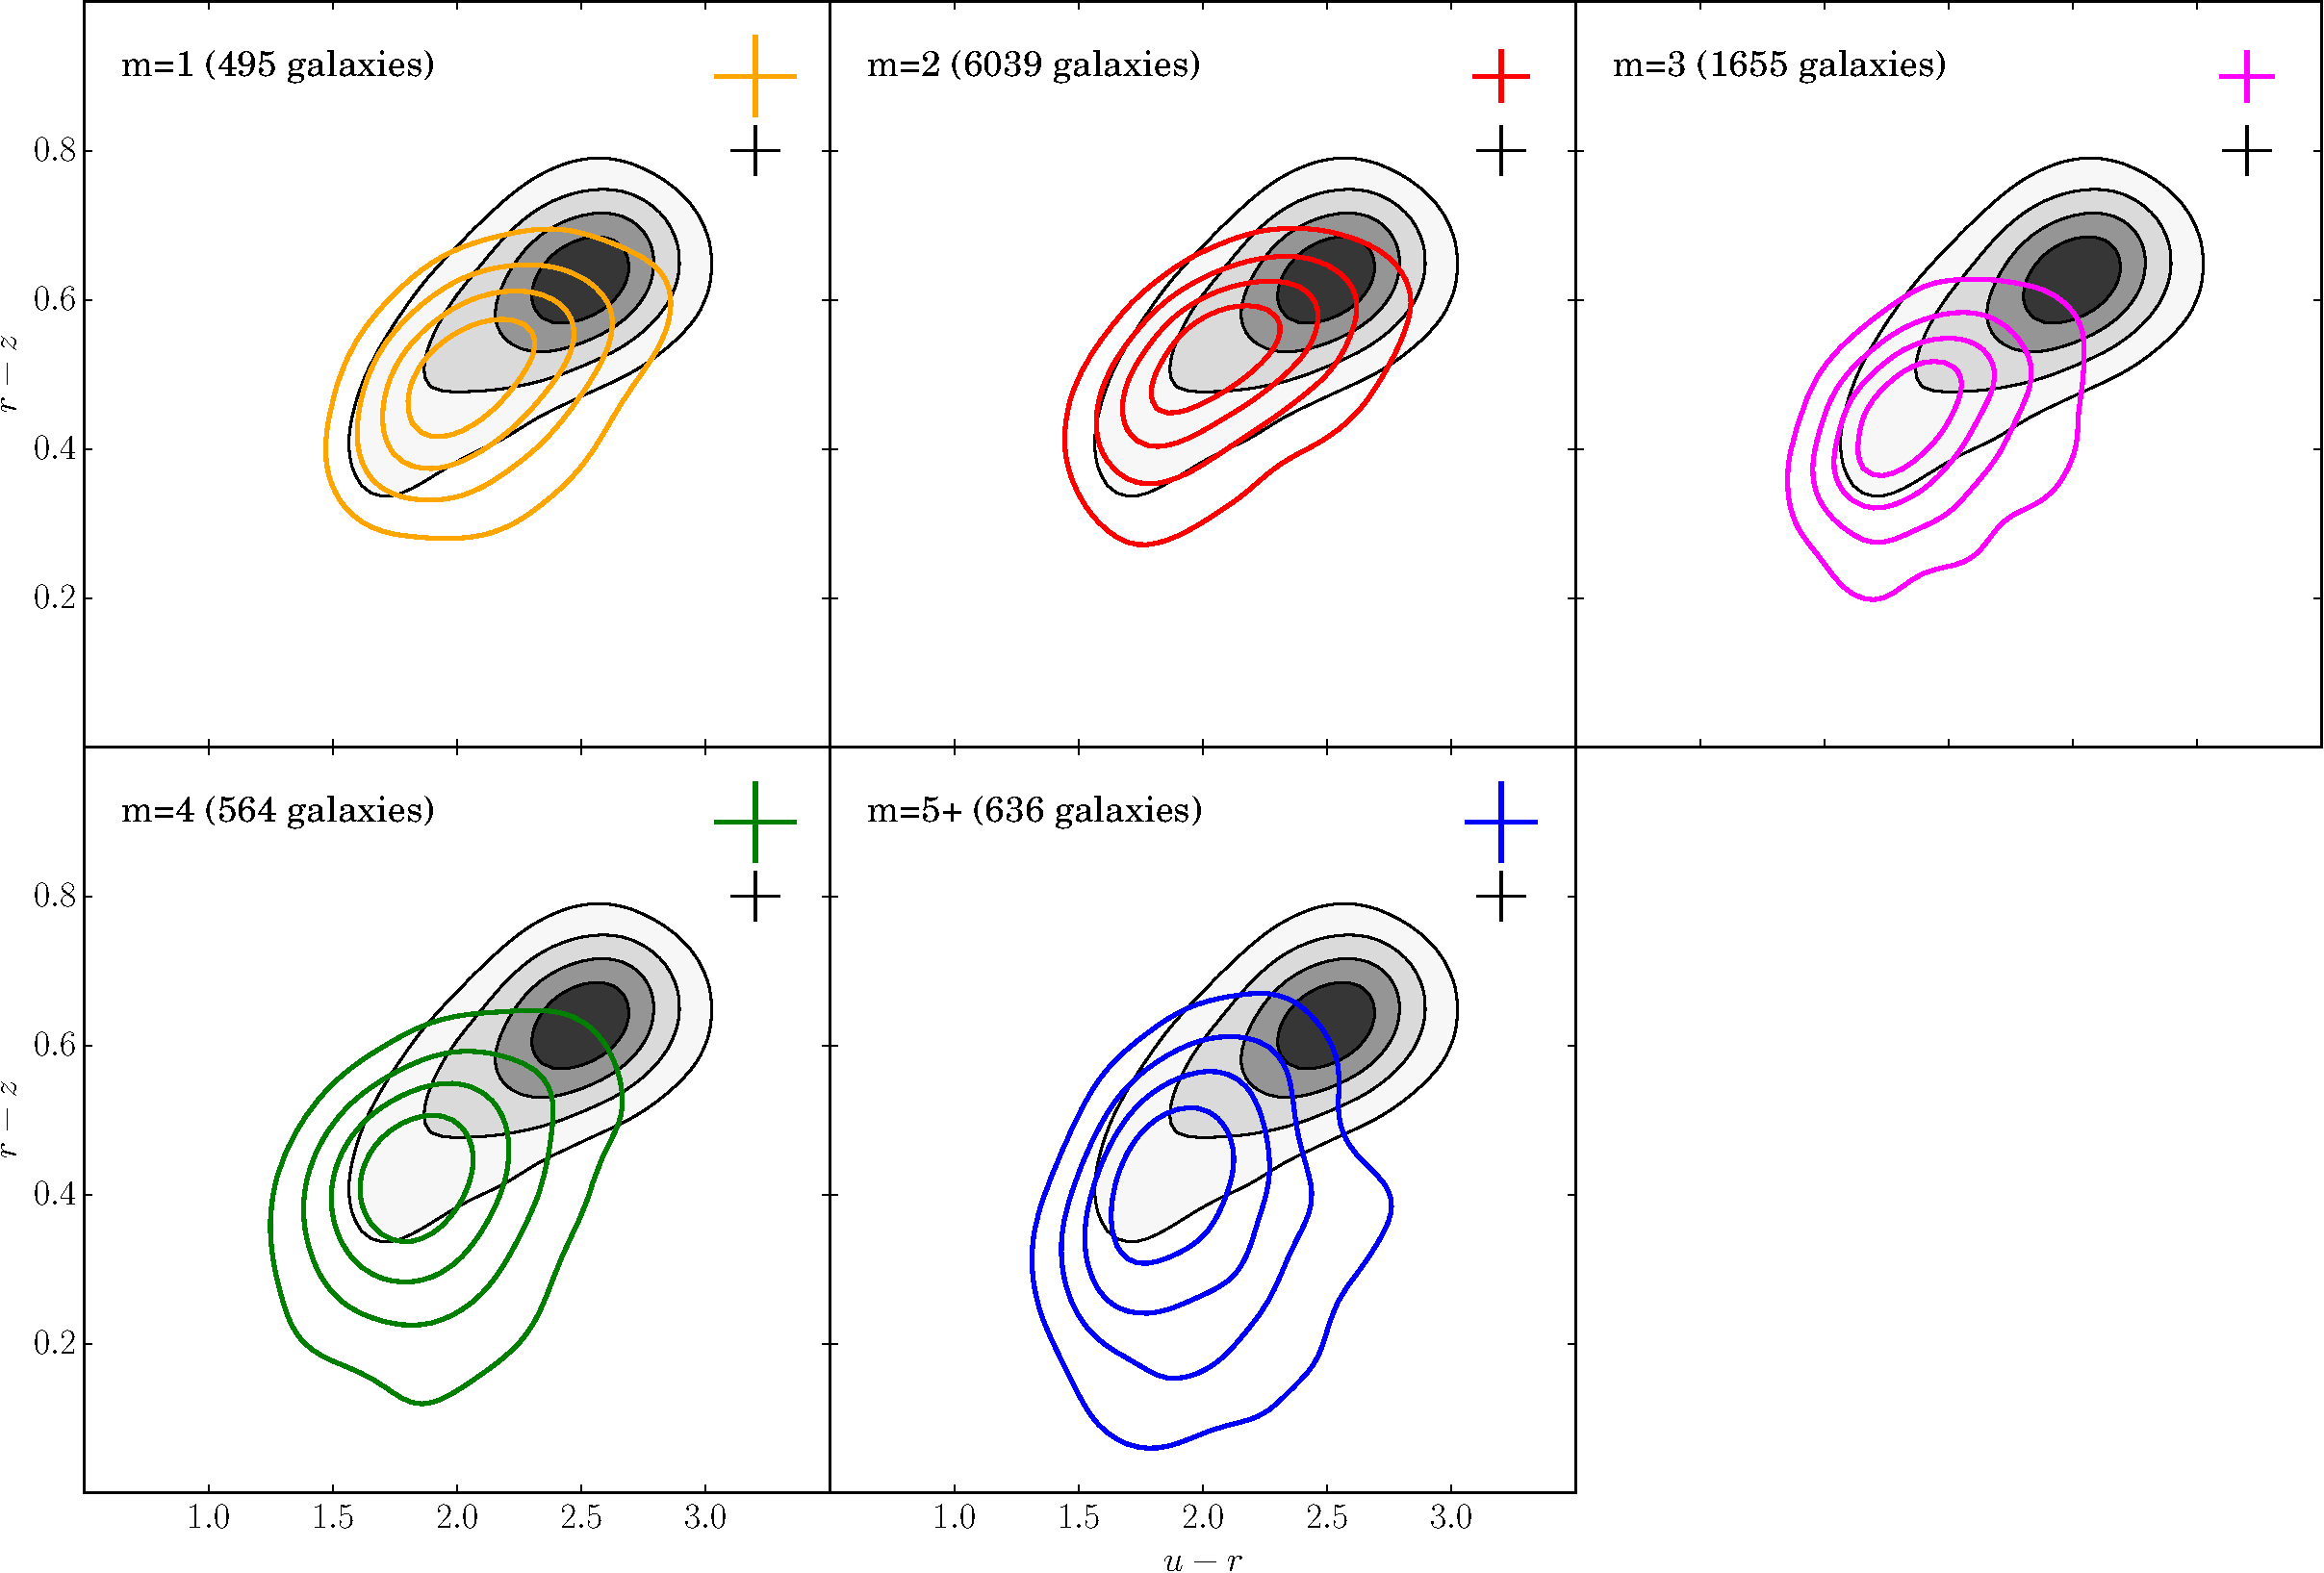
\includegraphics[width=0.975\textwidth]{Images/Results/cc1.pdf}

        \caption{$u-r$ vs. $r-z$ colours for each of the \textit{arm number samples} taken from the \textit{stellar mass limited spiral sample}. The greyscale shaded contours show the entire \textit{stellar mass-limited sample}, whereas the solid lines indicate the same distribution for each \textit{arm number sample}. The contours are plotted with a kernel density estimate, of bandwidth optimised using 5-fold cross validation, and the bandwidths are displayed in the top-left corner of each plot. The contour levels show the regions enclosing 20,40,60 and 80\% of the points.}

        \label{fig:colour-colour}

\end{figure*}

\begin{figure}
		\centering

        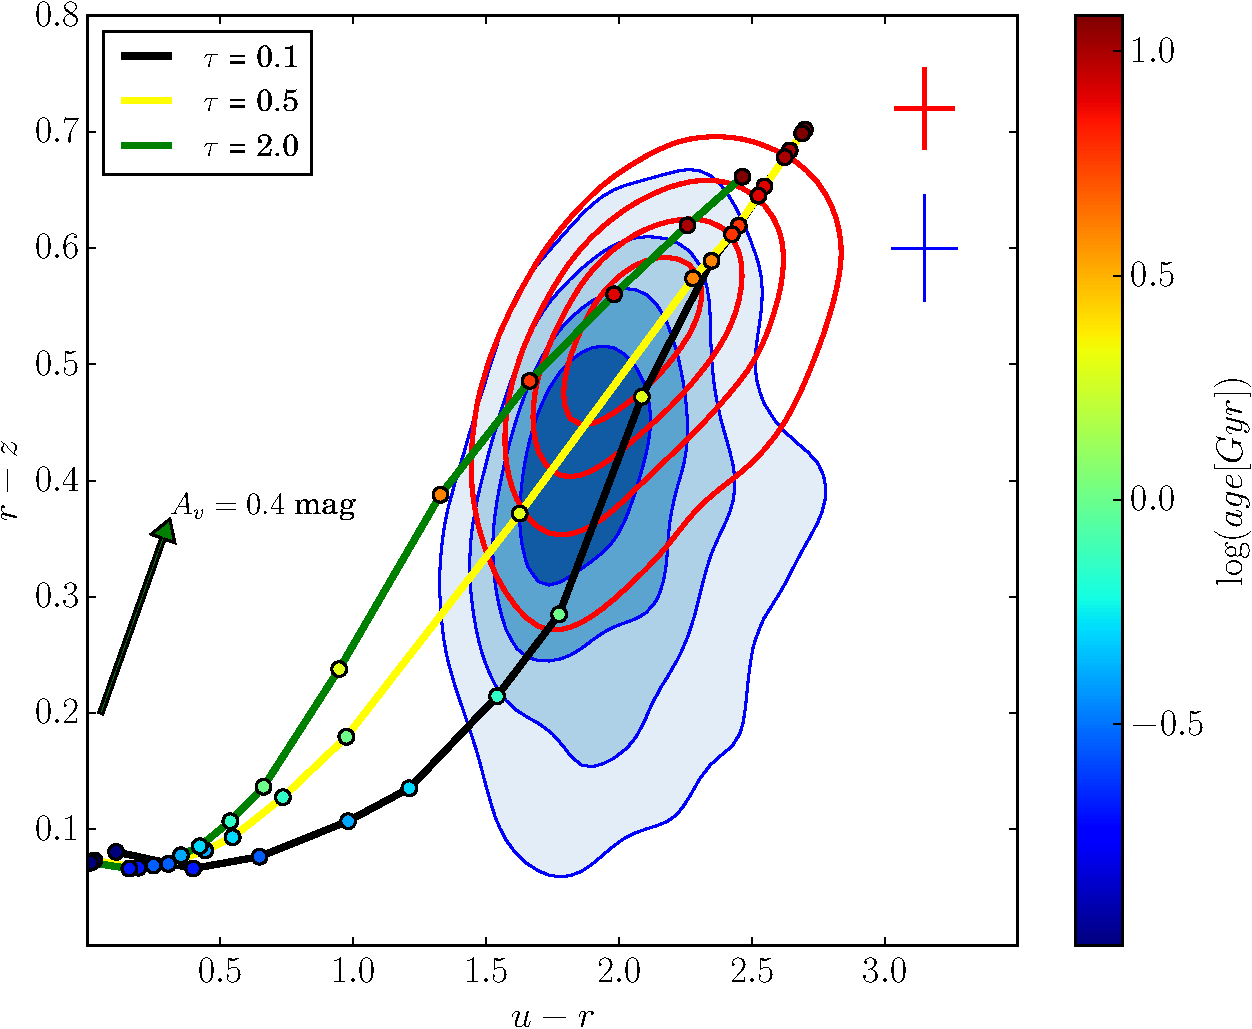
\includegraphics[width=0.45\textwidth]{Images/Results/cc1_w_sfh.pdf}

        \caption{Contour plots for the $m$=2 (red solid contours)and $m$=5+ (blue filled contours) samples as in Fig.~\ref{fig:colour-colour}. Three evolutionary tracks for $t$ and $\tau$ Bruzual \& Charlot models are also plotted in black, yellow and green lines, and the green arrow indicates how the respective lines would shift with dust extinction.}

        \label{fig:cc_w_sfh}

\end{figure}
%------------------------------------------------------------------------------------
%%%%%%%%%%%%%%%%%%%%%%%%%%%%%%%%%%%%%%%%%%%%%%%%%%%%%%%%%%%%%%%%%%%%%%%%%%%%%%%%%%%%%
%------------------------------------------------------------------------------------
\section{Conclusions}
\label{sec:conclusions}

In this paper, the overall demographics of a population of local spiral galaxies have been compared, in order to gain an understanding of any significant differences in the physical processes that play a role in the formation and evolution of spiral structure. Using visual classifications of SDSS galaxies from GZ2, a new debiasing procedure has been constructed, to make both the sample of spiral galaxies and the relative samples of galaxies with different spiral arm numbers as complete as possible.

Using these classifications, the overall demographics of environment, stellar mass and colour were compared. It was found that the most massive galaxies favour many-armed spiral structure. An enhancement in the fraction of two-armed spiral galaxies was observed in the highest density environments, indicating that galaxy-galaxy interactions could play a role in the inducement of two-armed spiral structure. The most significant differences between the galaxy populations were observed in terms of colour, where it was found that $m=2$ spiral galaxies could be either much dustier, or have undergone earlier quenching of star formation than in many-armed spiral galaxies. Combining these results, scenarios as to how spiral structure changes over a disk's lifetime can begin to be formulated. The earlier quenching could be indicative that two-armed spiral structure is a feature that occurs much later in a galaxy's lifetime, whereas multiple-armed structure happens much earlier. It could perhaps be the case that perturbations to the disk invoke two-armed spiral structure, which would be consistent with the SFH modeling and observed environmental trends. However, as the correlations with environment are relatively weak, it could also be the case that many-armed spiral structure `fades' to two-armed spiral structure via other mechanisms, such as growth of a strong bar or secular processes in the gas of the disk.

%------------------------------------------------------------------------------------
%%%%%%%%%%%%%%%%%%%%%%%%%%%%%%%%%%%%%%%%%%%%%%%%%%%%%%%%%%%%%%%%%%%%%%%%%%%%%%%%%%%%%
%------------------------------------------------------------------------------------

\section{Acknowledgements}

The data in this paper are the result of the efforts of the Galaxy Zoo 2 volunteers, without whom none of this work would be possible. Their efforts are individually acknowledged at authors.galaxyzoo.org.

\bibliographystyle{mn2e}
\bibliography{jun15}

\end{document}
